%% 
%% Copyright 2007-2025 Elsevier Ltd
%% 
%% This file is part of the 'Elsarticle Bundle'.
%% ---------------------------------------------
%% 
%% It may be distributed under the conditions of the LaTeX Project Public
%% License, either version 1.3 of this license or (at your option) any
%% later version.  The latest version of this license is in
%%    http://www.latex-project.org/lppl.txt
%% and version 1.3 or later is part of all distributions of LaTeX
%% version 1999/12/01 or later.
%% 
%% The list of all files belonging to the 'Elsarticle Bundle' is
%% given in the file `manifest.txt'.
%% 
%% Template article for Elsevier's document class `elsarticle'
%% with numbered style bibliographic references
%% SP 2008/03/01
%% $Id: elsarticle-template-num.tex 272 2025-01-09 17:36:26Z rishi $
%%
\documentclass[preprint,12pt]{elsarticle}
\usepackage{xcolor}
\usepackage{lineno}
%% Use the option review to obtain double line spacing
%% \documentclass[authoryear,preprint,review,12pt]{elsarticle}

%% Use the options 1p,twocolumn; 3p; 3p,twocolumn; 5p; or 5p,twocolumn
%% for a journal layout:
%% \documentclass[final,1p,times]{elsarticle}
%% \documentclass[final,1p,times,twocolumn]{elsarticle}
%% \documentclass[final,3p,times]{elsarticle}
%% \documentclass[final,3p,times,twocolumn]{elsarticle}
%% \documentclass[final,5p,times]{elsarticle}
%% \documentclass[final,5p,times,twocolumn]{elsarticle}

%% For including figures, graphicx.sty has been loaded in
%% elsarticle.cls. If you prefer to use the old commands
%% please give \usepackage{epsfig}

%% The amssymb package provides various useful mathematical symbols
\usepackage{amssymb}
%% The amsmath package provides various useful equation environments.
\usepackage{amsmath}
%% The amsthm package provides extended theorem environments
%% \usepackage{amsthm}
\usepackage{subcaption}
\usepackage{multirow}
\usepackage{tabularx}
\usepackage{placeins}
\usepackage{hyperref}
% --- 开始：优化图片排版参数 ---
\renewcommand{\topfraction}{0.9}      % 允许顶部图片占据页面的 90% (默认是 0.7)
\renewcommand{\bottomfraction}{0.8}   % 允许底部图片占据页面的 80%
\setcounter{topnumber}{2}             % 顶部允许放 2 张图
\setcounter{bottomnumber}{2}          % 底部允许放 2 张图
\setcounter{totalnumber}{4}           % 单页总共允许放 4 张图
\renewcommand{\dbltopfraction}{0.9}   % 双栏排版中顶部图片的限制
\renewcommand{\textfraction}{0.07}    % 页面上最少只需要保留 7% 的文字 (默认是 20%)
\renewcommand{\floatpagefraction}{0.7} % 只有当图片占满单独一页的 70% 时，才允许单独成页
% --- 结束：优化图片排版参数 ---

\newcommand*{\mkblue}[1]{{\color{blue}{#1}}}
\newcommand{\doi}[1]{\url{https://doi.org/#1}}
\linenumbers
%% The lineno packages adds line numbers. Start line numbering with
%% \begin{linenumbers}, end it with \end{linenumbers}. Or switch it on
%% for the whole article with \linenumbers.
%% \usepackage{lineno}

\journal{Astroparticle Physics}

\begin{document}

\begin{frontmatter}

%% Title, authors and addresses

%% use the tnoteref command within \title for footnotes;
%% use the tnotetext command for theassociated footnote;
%% use the fnref command within \author or \affiliation for footnotes;
%% use the fntext command for theassociated footnote;
%% use the corref command within \author for corresponding author footnotes;
%% use the cortext command for theassociated footnote;
%% use the ead command for the email address,
%% and the form \ead[url] for the home page:
%% \title{Title\tnoteref{label1}}
%% \tnotetext[label1]{}
%% \author{Name\corref{cor1}\fnref{label2}}
%% \ead{email address}
%% \ead[url]{home page}
%% \fntext[label2]{}
%% \cortext[cor1]{}
%% \affiliation{organization={},
%%             addressline={},
%%             city={},
%%             postcode={},
%%             state={},
%%             country={}}
%% \fntext[label3]{}

\title{
   %Cosmic ray electrons' trajectory reconstruction for the DAMPE BGO calorimeter using a physics-guided deep learning strategy up to 90 degrees on zenith
   Hierarchical Deep Learning for Zenith-to-Horizon Electron Trajectory Reconstruction in the DAMPE BGO Calorimeter
   \mkblue{Hierarchical Deep Learning for BGO-Only Electron Track Reconstruction with DAMPE}
}

%% use optional labels to link authors explicitly to addresses:
%% \author[label1,label2]{}
%% \affiliation[label1]{organization={},
%%             addressline={},
%%             city={},
%%             postcode={},
%%             state={},
%%             country={}}
%%
%% \affiliation[label2]{organization={},
%%             addressline={},
%%             city={},
%%             postcode={},
%%             state={},
%%             country={}}

 \author[inst1,inst2]{Xun Zhu}
% \ead{1224046031@njupt.edu.cn}

\author[inst2]{PengXiong Ma}
\ead{mapx@pmo.ac.cn}


 \author[inst2,inst3]{JianHua Guo}
\author[inst2,inst3]{Xiang Li}

 \affiliation[inst1]{organization={School of Computer Science, Nanjing University of Posts and Telecommunications},
             city={Nanjing},
             country={China}}

 \affiliation[inst2]{organization={Key Laboratory of Dark Matter and Space Astronomy, Purple Mountain Observatory, Chinese Academy of Sciences},
             city={Nanjing},
             country={China}}

 \affiliation[inst3]{organization={School of Astronomy and Space Science, University of Science and Technology of China},
             city={Hefei},
             country={China}}



%% Abstract
\begin{abstract}
%% Text of abstract
Reliable track reconstruction is fundamental to the Dark Matter Particle Explorer (DAMPE) mission, as the determination of multiple cosmic ray properties relies heavily on precise trajectory information. Conventional reconstruction algorithms focus primarily on penetrating events, effectively leveraging measurements from the Silicon-Tungsten Tracker (STK) and the BGO calorimeter, with the STK providing the critical anchor for track precision. However, for large-angle incident events---particularly those traversing the BGO calorimeter quasi-horizontally---the absence of reliable STK measurements renders traditional methods ineffective. To unlock DAMPE's observational potential at large angles, specifically for electron-like cosmic rays, we propose a hierarchical deep learning framework relying solely on BGO shower profiles in this work. To ensure robust application to unlabeled flight data, we introduce a Support Vector Machine (SVM) classifier to reliably distinguish between standard-angle ($0^{\circ}$--$60^{\circ}$) and large-angle ($60^{\circ}$--$90^{\circ}$) regimes based on distinct shower morphologies. Accordingly, we develop specialized models adapted to each interval: a physics-guided hybrid model fusing the DAMPE energy-weighted Center-of-Gravity reconstruction with deep learning for standard angles, and a deep-learning-dominant strategy to recover trajectories from truncated showers in the STK-blind region. Validated on Monte Carlo datasets, our method achieves nearly 100\% reconstruction efficiency across the full angular range, with an angular resolution (68\% containment radius) of $1.40^{\circ}$ for standard angles and $1.31^{\circ}$ for large angles. A cross-check on flight electron candidates with STK tracks ($30^{\circ}$--$71^{\circ}$) shows degree-level agreement between the BGO-only predictions and the STK reference directions (median angular difference $1.44^{\circ}$, 68th percentile $1.98^{\circ}$). By extending reliable reconstruction into the $60^{\circ}$--$90^{\circ}$ band where the STK is unavailable, this work raises the effective acceptance of the detector by a factor of 1.8.
\end{abstract}

%%Graphical abstract
%\begin{graphicalabstract}
%\includegraphics{grabs}
%\end{graphicalabstract}

%%Research highlights
%\begin{highlights}
%\item Research highlight 1
%\item Research highlight 2
%\end{highlights}

%% Keywords
\begin{keyword}
Particle Track Reconstruction \sep Deep Learning \sep BGO Calorimeter \sep Large-Angle Events
\end{keyword}

\end{frontmatter}

%% Add \usepackage{lineno} before \begin{document} and uncomment 
%% following line to enable line numbers

%% main text
%%

%% Use \section commands to start a section
\section{Introduction}
\label{sec:intro}

The Dark Matter Particle Explorer (DAMPE), launched in December 2015, is a high-energy cosmic-ray and gamma-ray observatory operating in a sun-synchronous orbit~\cite{dampe_mission}. Its primary scientific objectives include the indirect search for dark matter, the precise measurement of cosmic-ray spectra (electrons~\cite{ambrosi_2017}, protons~\cite{an_2019}, helium~\cite{alemanno_helium_2021,alemanno_p_he_2024}, and heavier nuclei~\cite{alemanno_proton_iron_2025}) up to the PeV scale, and high-energy gamma-ray astronomy~\cite{li_2019}. To fulfill the stringent requirements for precise energy measurement and particle identification, the DAMPE payload comprises four sub-detectors: a Plastic Scintillator Detector (PSD)~\cite{dampe_psd_calib, dampe_psd_design, dong_2019, ma_2019}, a Silicon-Tungsten Tracker (STK)~\cite{dampe_stk_perf, dampe_stk_align, dampe_stk_design}, a Bismuth Germanium Oxide (BGO) imaging calorimeter~\cite{dampe_bgo_beam, dampe_bgo_calib, dampe_bgo_readout}, and a Neutron Detector (NUD)~\cite{dampe_nud}.

In the standard reconstruction pipeline adopted by the DAMPE collaboration, precise trajectory reconstruction relies heavily on the synergy between the BGO calorimeter and the STK~\cite{dampe_stk_soft}, a design philosophy shared by major space-borne experiments such as Fermi-LAT~\cite{atwood_2009} and CALET~\cite{asaoka_2019, asaoka_cal_2017}. Typically, the shower axis is first coarsely estimated using the BGO energy distribution, which then seeds the search for track candidates in the STK. The STK, with its fine silicon strips, supplies the precise angular measurement that, together with the BGO seed, yields a trajectory resolution of approximately $0.2^{\circ}$ at 10 GeV for the combined BGO+STK pipeline~\cite{dampe_stk_perf}. This trajectory is then projected back to the PSD for absolute charge measurement. Although this multi-detector synergy yields high precision, it suffers from an intrinsic geometric limitation: the incident particle must traverse the fiducial volumes of the PSD, STK, and BGO simultaneously.

Due to the limitations of the aspect ratio and trigger logic of the DAMPE payload~\cite{dampe_trigger_2019}, events with zenith angles exceeding $\sim 60^{\circ}$ often bypass the fiducial volumes of the PSD and STK, or traverse only limited layers of STK, which is insufficient to form a track candidate. Consequently, the standard Kalman-filter-based tracking algorithms become inapplicable~\cite{dampe_stk_soft}. For scientific goals that require high statistics, such as the search for monochromatic gamma-ray lines~\cite{liang_2022} or the precise measurement of rare high-energy spectral features, maximizing the effective field of view is paramount. Therefore, the development of a trajectory reconstruction method that relies exclusively on the BGO calorimeter, the key sub-detector with a sufficiently large acceptance to capture these events, is essential.

\begin{figure}[htbp]
\centering
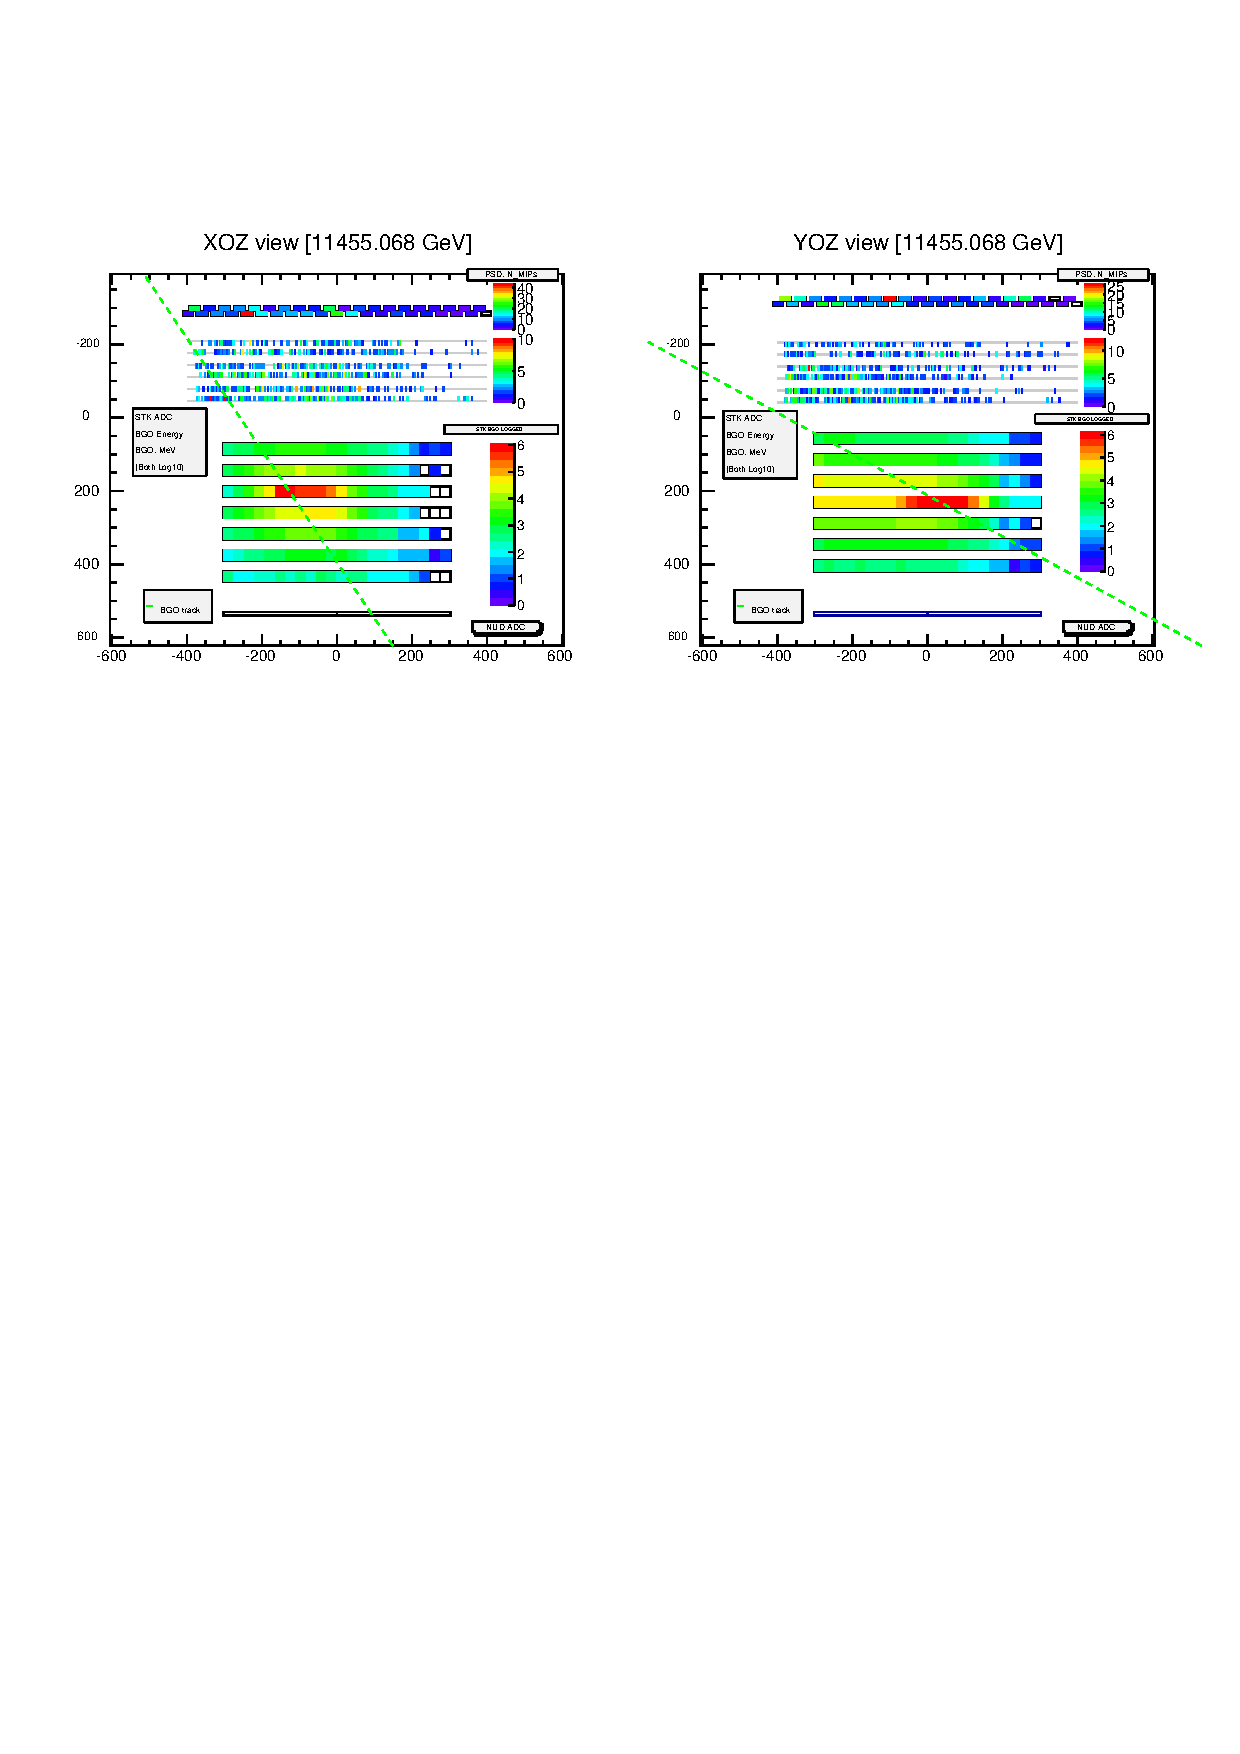
\includegraphics[width=\columnwidth,trim=20 480 20 10,clip]{graph/fig1.pdf}
\caption{Schematic of the geometric limitation. The green dashed line illustrates the BGO-only track reconstructed by the Standard BGO Algorithm, representing a large-angle trajectory that traverses the BGO calorimeter but bypasses the PSD and STK detectors.}
\label{fig:limitation}
\end{figure}

Reconstructing trajectories using only the BGO calorimeter is difficult, particularly for large-angle events. The standard BGO reconstruction is the official DAMPE energy-weighted Center-of-Gravity (CoG) track reconstruction~\cite{dampe_bgo_reco_status, lei_2019}, hereafter the Standard BGO Algorithm; it reconstructs the shower axis from the energy-weighted centroids of the BGO layers. While effective for showers that are fully contained within the calorimeter, this analytical approach degrades once the incident angle grows large, as shown in Figure~\ref{fig:limitation}. As the incident angle increases, the electromagnetic or hadronic showers are often not fully contained within the calorimeter depth. This phenomenon, known as ``side leakage,'' causes a systematic shift in the energy-weighted centroid of the shower development, leading to substantial biases in the reconstructed direction. In addition, the limited number of BGO layers traversed by large-angle particles reduces the available information for fitting, rendering the CoG track fit unstable and unreliable.

Deep learning has been widely applied with success to calorimeter shower analysis in high-energy physics~\cite{paganini_2018, erdmann_2018, guillen_2019, yang_2024, carleo_2019, seyyedi_2023, meng_2025, lecun_2015}. For the DAMPE experiment, Tykhonov et al.~\cite{tykhonov_2023} successfully applied Convolutional Neural Networks (CNNs) to improve the BGO shower axis prediction, providing a superior seed for the STK. However, existing works have largely focused on optimizing performance within the standard geometric acceptance, that is, improving the resolution of events that can be observed by the STK, rather than extending reconstruction into the large-angle regime where the STK is unavailable. The present method instead operates on BGO data alone to recover events in the $60^{\circ}$--$90^{\circ}$ band that the STK-dominated pipeline discards, complementing rather than competing with STK-based reconstruction.

The approach in this work tailors the reconstruction logic to the physical shower morphology at each incident angle. For the standard-angle regime, we embed physical principles and geometric features directly into the neural network architecture, ensuring that the model adheres to known physical laws during the learning process. This physics-informed feature engineering coupled with a physics-gated hybrid fusion can be viewed as a ``gray-box'' model~\cite{karpatne_2017, kerrigan_2021, karniadakis_2021, willard_2022}: it keeps predictions consistent with known physical constraints while retaining the representational power of deep learning. For the large-angle regime, where physical priors become unreliable due to severe side leakage, we adopt a Deep-Learning-Dominant(DLD) strategy that relies on enhanced input representation and multi-task learning to recover trajectory information from truncated showers. We further developed a Support Vector Machine (SVM)~\cite{cortes_1995} classifier to automatically categorize events into ``standard-angle'' ($0^{\circ}$--$60^{\circ}$) and ``large-angle'' ($60^{\circ}$--$90^{\circ}$) regimes based on shower morphology, thereby enabling the processing of unlabeled flight data.

The organization of the paper is as follows: Section ~\ref{sec:data} presents the simulation data, Section ~\ref{sec:method} introduces and implements the methods, Section ~\ref{sec:eval} covers performance evaluation, and discussion and conclusion are provided in Sections ~\ref{sec:discussion} and ~\ref{sec:conclusion}, respectively.


\section{Data and Simulation}
\label{sec:data}

The DAMPE detector consists of four sub-detectors.
Among these, the BGO calorimeter is the primary instrument for energy measurement and is central to electron-hadron discrimination. It is composed of 308 BGO crystal bars, each measuring $2.5 \times 2.5 \times 60 \text{ cm}^3$. These bars are arranged in 14 layers, with each layer containing 22 bars~\cite{dampe_mission, dampe_bgo_calib}. The layers are stacked in an orthogonal hodoscopic configuration, in which odd-numbered layers are oriented along the Y-axis and even-numbered layers along the X-axis. This design provides a total depth of approximately 31 radiation lengths and allows for three-dimensional tomographic reconstruction of the particle shower development. The geometric arrangement of the BGO bars naturally maps to a $14 \times 22$ grid, which is the foundational data structure for the deep learning model.

To train and validate the proposed deep learning framework, a large-scale dataset was generated using the GEANT4~\cite{geant4_2016} simulation toolkit. The simulation incorporates a detailed model of the DAMPE detector geometry~\cite{dampe_stk_soft} and material properties, along with extensive physics lists for particle interactions~\cite{ftfp_model1, ftfp_model2, bertini_cascade}. The dataset focuses on electron events, which are the primary targets of this work and can be separated from hadronic showers using BGO data alone. The detailed simulation parameters are configured as follows:
\begin{itemize}
    \item \textbf{Particle Type}: Electrons ($e^-$).
    \item \textbf{Energy Range}: 100 GeV to 1 TeV, following a power-law spectrum with a spectral index of $-1.0$ to ensure sufficient statistics at high energies.
    \item \textbf{Angular Distribution}: The incident particles were generated on a sphere of radius 1.38\,m centred on the detector axis, 24.7\,cm above the geometric centre of the BGO calorimeter, with an isotropic angular distribution covering the full zenith angle range from $0^{\circ}$ to $90^{\circ}$; this radius is referred to as the generation radius. This full-angle coverage is essential for training the model to handle large-angle events that are typically discarded by standard selection criteria.
    \item \textbf{Total Statistics}: A total of 11,894,154 events were selected. The dataset was randomly split into training (80\%) and testing (20\%) sets.
\end{itemize}

The two expert branches are trained on overlapping angular sub-ranges of
this sample ($0^{\circ}$--$70^{\circ}$ and $50^{\circ}$--$90^{\circ}$);
the 80/20 train/test partition is unchanged.

To facilitate efficient learning by the neural network, we perform a series of pre-processing steps to construct two distinct input streams: the BGO Energy Map and the Physics-informed Feature Vector. The energy deposition in the 308 BGO bars is mapped into a $14 \times 22$ matrix, in which each element $(i, j)$ represents the energy deposited in the $j$-th bar of the $i$-th layer. Although this projection flattens the three-dimensional detector geometry into a two-dimensional grid, the orthogonal hodoscopic nature of the calorimeter is implicitly preserved in the row-wise structure (alternating X and Y orientations). This allows the model to learn spatial correlations specific to the cross-layered topology of the detector. To handle the large dynamic range of energy deposits (spanning from GeV to TeV) and to normalize the input distribution, we construct a dual-channel input tensor of shape $(14, 22, 2)$:
\begin{enumerate}
    \item \textbf{Normalized Energy Channel}: To capture the relative shower shape independent of the absolute energy scale, the energy in each bar is normalized by the total energy deposited in the event:
    \begin{equation}
    E_{\text{norm}}^{(i,j)} = \frac{E^{(i,j)}}{\sum_{i,j} E^{(i,j)}}
    \end{equation}
    \item \textbf{Log-transformed Energy Channel}: To preserve information about low-energy deposits tracing the shower periphery while compressing the high-energy core, we apply a logarithmic transformation:
    \begin{equation}
    E_{\text{log}}^{(i,j)} = \ln(1 + E^{(i,j)})
    \end{equation}
\end{enumerate}

In addition to the raw energy map, we extract a 24-dimensional vector of physics-based features to guide the network. These features encapsulate domain knowledge about electromagnetic shower development and provide explicit physical guidance to the network. The features are categorized as follows:
\begin{enumerate}
    \item \textbf{Layer-wise Energy Distribution (7 features)}: The total energy deposited in each of the 7 X-Y layer pairs. This describes the longitudinal profile of the shower.
    \item \textbf{Layer-wise Maximum Energy (7 features)}: The average of the maximum energy deposition in the X and Y bars for each layer pair, indicating the intensity of the shower core. 
    \item \textbf{Layer-wise Maximum-Energy Bar Position (7 features)}: For each layer pair, the average bar index of the X and Y bars that record the maximum energy deposition, providing a coarse estimate of the shower axis in that layer.
    \item \textbf{Global Energy-Weighted Centroid (3 features)}: The energy-weighted mean position $(X_c, Y_c, Z_c)$ of the entire shower in the detector coordinate system. This is calculated as:
    \begin{equation}
    X_c = \frac{\sum_{i,j} x_{i,j} \cdot E_{i,j}}{\sum_{i,j} E_{i,j}}, \quad Y_c = \frac{\sum_{i,j} y_{i,j} \cdot E_{i,j}}{\sum_{i,j} E_{i,j}}, \quad Z_c = \frac{\sum_{i,j} z_{i,j} \cdot E_{i,j}}{\sum_{i,j} E_{i,j}}
    \end{equation}
    where $(x_{i,j}, y_{i,j}, z_{i,j})$ are the spatial coordinates of the $j$-th bar in the $i$-th layer.
\end{enumerate}
These 24 features serve as explicit physical constraints for the standard-angle branch; the exact composition of the physics vector is regime-specific, and the large-angle variant is detailed in Section~\ref{ssec:large}.


\FloatBarrier
\section{Methodology}
\label{sec:method}

We now detail the architecture of this hierarchical framework.

\subsection{Overall Framework}
\label{ssec:framework}

Electromagnetic showers in the BGO calorimeter develop differently depending on the incident angle. To effectively address these variations, we categorize incident events into two distinct regimes: the standard-angle regime ($0^{\circ}$--$60^{\circ}$) and the large-angle regime ($60^{\circ}$--$90^{\circ}$), also referred to as standard and large incidence. This categorization is empirically determined by two independent facts that happen to coincide near $60^{\circ}$: the geometric acceptance of the DAMPE detector, which removes the STK from the measurement above this angle, and the degradation of the Standard BGO Algorithm at large incidence. Monte Carlo simulations demonstrate that the reconstruction efficiency of the Standard BGO Algorithm remains acceptable for zenith angles up to approximately $60^{\circ}$, but drops steeply beyond this threshold (Section~\ref{ssec:efficiency}). The two are physically distinct. Above $60^{\circ}$ the shower is frequently not contained within the calorimeter depth, so side leakage biases the energy-weighted centroid and the CoG fit degrades; independently, particles at these angles typically bypass the fiducial volume of the STK, leaving the BGO calorimeter as the sole source of trajectory information. Consequently, events in the standard-angle regime are typically well-contained, exhibiting clear longitudinal and lateral profiles. Conversely, events in the large-angle regime suffer from severe side leakage and truncated path lengths, producing truncated, irregular shower topologies that require a specialized deep-learning strategy.

To accommodate these distinct physical regimes, we design a two-branch pipeline:

\begin{enumerate}
    \item \textbf{Zenith Categorization}: An incoming event is first processed by SVM classifier to obtain its approximate incident‑angle range.
    \item \textbf{Model Selection}: Based on the above classification, the event is routed to either the standard-angle Branch (utilizing a physics-guided hybrid strategy) or the large-angle Branch (utilizing a deep-learning-dominant strategy), irrespective of the wider angular range used in training.
\end{enumerate}

This hierarchical structure ensures that the reconstruction algorithm is optimal for the specific topology of the event, balancing robustness and precision. 

\subsection{Angle Classifier}
\label{ssec:classifier}

Since flight data lack ground-truth labels for incident angles, an automatic categorization mechanism is a prerequisite for the hierarchical framework. We developed a classifier based on a Support Vector Machine (SVM)~\cite{cortes_1995, pedregosa_2011} to distinguish between standard-angle and large-angle events from shower morphology alone.

\textbf{Input representation.} Rather than feeding the full 308-dimensional raw energy vector, the classifier operates on a compact 7-dimensional physics feature vector extracted from the $14\times22$ BGO energy matrix. Writing $E_{l,b}$ for the energy in bar $b$ of layer $l$ and $E_l=\sum_b E_{l,b}$ for the layer energy, the vector combines three geometric descriptors with four basic shower quantities:
\begin{itemize}
\item \textbf{Longitudinal (depth) RMS} ($\sigma_{\rm long}$, in \emph{layer} units) --- the energy-weighted Root Mean Square (RMS) spread of the layer index:
\begin{equation}
\textstyle
\sigma_{\rm long}=\Big[\sum_l (l-\bar l)^2E_l \big/ \sum_l E_l\Big]^{1/2},
\quad
\bar l=\sum_l lE_l \big/ \sum_l E_l
\end{equation}
\item \textbf{Lateral RMS width} ($\sigma_{\rm lat}$, in \emph{bar} units) --- the average over the 14 layers of the energy-weighted RMS spread of the bar index within each layer:
\begin{equation}
\textstyle
\sigma_{\rm lat}=\tfrac{1}{14}\sum_l\Big[\sum_b (b-\bar b_l)^2E_{l,b} \big/ \sum_b E_{l,b}\Big]^{1/2},
\quad
\bar b_l=\sum_b bE_{l,b} \big/ \sum_b E_{l,b}
\end{equation}
\item \textbf{Shower-axis slope magnitude} ($s_{\rm mag}$, in \emph{bar units per layer}, numerically close to the tangent of the shower tilt) --- the energy-weighted linear regression of each layer's transverse centroid against the layer index, performed separately for the $X$-view (even layers) and the $Y$-view (odd layers) and combined as
\begin{equation}
\textstyle
s_{\rm mag}=\sqrt{s_x^2+s_y^2}
\end{equation}
\item \textbf{Four basic quantities} --- the layer of maximum energy deposition, the total deposited energy, and the two individual slope projections $|s_x|$ and $|s_y|$.
\end{itemize}
All quantities are expressed in the detector's native bar/layer indices rather than physical distances, keeping them scale-free and directly observable in unlabeled flight data, and together they capture the essential morphological differences between standard and large-angle showers.

\textbf{Model and training.} We use a scikit-learn Support Vector Classifier(SVC) with an Radial Basis Function(RBF) kernel ($C=10$, $\gamma=\texttt{scale}$), preceded by a \texttt{StandardScaler} for $z$-score normalization of the input features. The classifier is trained on a class-balanced sample of 50,000 Monte Carlo events drawn from a stratified pool of 300,000 events, using an 80/20 train/test partition; events are labeled by the true incident-angle threshold $\theta>60^{\circ}$. On the held-out test set the classifier reaches an accuracy of 98.4\%.

\textbf{Characterization and failure modes.} Table~\ref{tab:svm} reports the per-class \textbf{precision}, \textbf{recall}, and \textbf{F1 score}; both regimes are well balanced. The two metrics answer complementary questions and differ only in their denominator. Taking the large-angle class as an example, let TP be the number of genuinely large-angle events that the classifier also labels large-angle, FP the number of standard-angle events it mislabels as large-angle, and FN the number of genuinely large-angle events it mislabels as standard-angle. \textbf{Precision} $=\mathrm{TP}/(\mathrm{TP}+\mathrm{FP})$ asks, \emph{of all events the classifier flags as large-angle, how many really are?} It measures the \emph{purity} of the routing. \textbf{Recall} $=\mathrm{TP}/(\mathrm{TP}+\mathrm{FN})$ asks, \emph{of all genuinely large-angle events, how many does the classifier find?} It measures the \emph{completeness}. The \textbf{F1 score} is their harmonic mean, balancing purity against completeness. For instance, of 10,000 events flagged as large-angle about 9,820 truly are (precision 0.982), while of 10,000 genuine large-angle events about 9,800 are correctly flagged (recall 0.980). In routing terms, a precision loss lets the wrong shower type contaminate a branch, whereas a recall loss discards genuine events into the wrong expert; since both experts are trained on overlapping ranges straddling the $60^{\circ}$ boundary and perform comparably there (Section~\ref{ssec:boundary}), either error affects the final resolution only marginally. Misclassified events are concentrated near the $60^{\circ}$ decision boundary. To quantify the impact of imperfect routing on the final angular resolution, we perform a routing ablation in which the learned classifier is replaced by an oracle (perfect) router: this changes the global $\Psi_{68}$ by only $0.03^{\circ}$, indicating that residual misrouting does not dominate the reconstruction error budget. Because the boundary region ($55^{\circ}$--$60^{\circ}$) is where the two expert models exhibit comparable performance (Section~\ref{ssec:boundary}), a misrouted event in this narrow band incurs at most a $0.06^{\circ}$ degradation, which is small relative to the overall resolution. The SVM is therefore a reliable, autonomous routing module.%: it is the component that would translate the theoretical performance of the deep learning models into a practical pipeline for processing the continuous stream of raw data downlinked from the satellite.

\begin{table}[htbp]
\centering
\caption{Performance of the SVM angle classifier on the held-out test set.}
\label{tab:svm}
\begin{tabular*}{\textwidth}{@{\extracolsep{\fill}}lccc}
\hline
\textbf{Class} & \textbf{Precision} & \textbf{Recall} & \textbf{F1} \\ \hline
Standard-angle ($0^{\circ}$--$60^{\circ}$) & 0.988 & 0.986 & 0.987 \\
Large-angle ($60^{\circ}$--$90^{\circ}$) & 0.982 & 0.980 & 0.981 \\ \hline
Overall accuracy & \multicolumn{3}{c}{98.4\%} \\ \hline
\end{tabular*}
\end{table}

\subsection{Reconstruction for Standard Incidence}
\label{ssec:standard}

For particles falling within the standard regimes ($0^{\circ}$--$60^{\circ}$), the shower profiles are generally complete and well-contained within the BGO calorimeter. In this regime, the official energy-weighted CoG reconstruction provides a physically robust, albeit sometimes imprecise, baseline~\cite{dampe_bgo_reco_status, lei_2019}. To exploit the complementary strengths of both approaches, we employ a Physics-Guided Hybrid Neural Network (PGHNN).

\begin{figure}[!t]
\centering
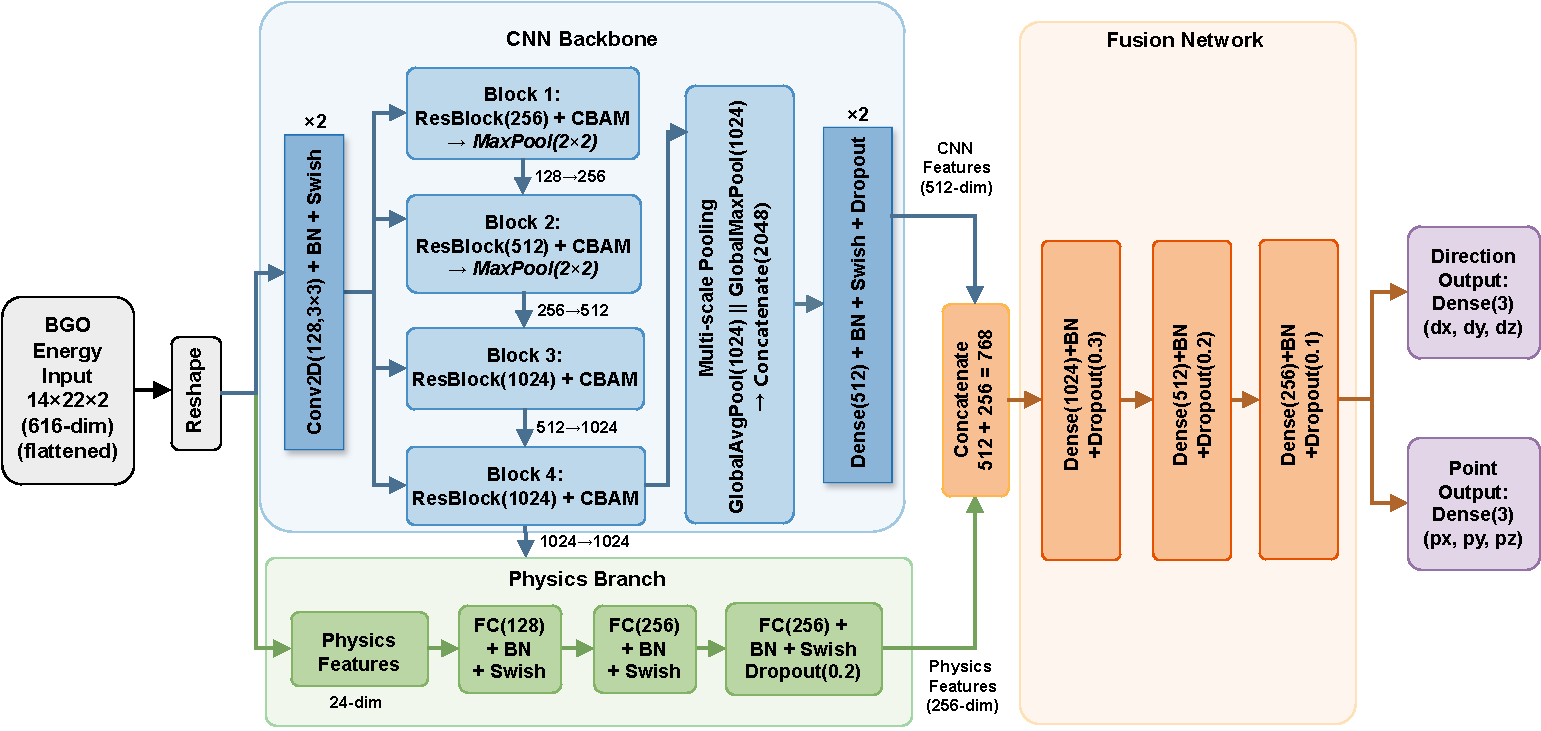
\includegraphics[width=0.8\textwidth]{graph/standard_architecture_new.pdf}
\caption{Schematic overview of the Physics-Guided Hybrid Neural Network (PGHNN) for standard-angle events ($0^{\circ}$--$60^{\circ}$). The architecture features a dual-stream structure processing BGO energy maps (2-channel input) and physics features, feeding a fusion network that drives two output heads: a direction head $\vec{D}_{\text{dl}}$ (\texttt{Dense(3)}) and a point head $\vec{P}_{\text{dl}}$ (\texttt{Dense(3)}). At inference the final trajectory is obtained by fusing the deep-learning prediction with the analytic (Standard BGO Algorithm) reconstruction through a gate $I_{\text{valid}}$ derived from the validity of the analytic fit.}
\label{fig:pghnn_arch}
\end{figure}

\textbf{Input Representation:} The PGHNN takes a 2-channel input tensor of shape $(14, 22, 2)$: (1) the per-event normalized energy channel $E_{ij}/\sum E$ capturing relative shower shape, and (2) the log-transformed energy channel $\ln(1+E_{ij})$ preserving low-energy periphery details (Section~\ref{sec:data}). This flat $616$-dimensional vector is reshaped to $(14,22,2)$ by a dedicated \texttt{BGOInput} layer.

\textbf{Architecture and Mechanism:} As illustrated in Figure~\ref{fig:pghnn_arch}, the PGHNN has a dual-stream architecture designed to process heterogeneous data.
\begin{enumerate}
    \item \textbf{CNN Stream:} The reshaped BGO energy map is processed by two initial Conv2D layers with 128 filters each, each followed by batch normalization and a Swish activation, and then by four residual blocks~\cite{he2016deep} equipped with Convolutional Block Attention Modules (CBAM)~\cite{woo2018cbam} at increasing depths (256, 512, 1024, 1024 filters); the first two blocks are followed by $2\times2$ max-pooling while the last two are not. Multi-scale pooling~\cite{szegedy2016rethinking} (GlobalAveragePooling and GlobalMaxPooling, each over the 1024-channel feature maps) is concatenated into a 2048-dimensional vector, which is compressed through two \texttt{Dense(512)} layers with batch normalization, Swish and dropout into a 512-dimensional CNN feature vector.
    \item \textbf{Physics Stream:} Simultaneously, the 24-dimensional physics feature vector is processed by a fully connected network with layers of 128, 256, and 256 neurons (each followed by batch normalization and Swish, with the final layer additionally applying dropout of $0.2$).
\end{enumerate}
These two streams are concatenated ($768$ dimensions) and fed into a fusion network (1024--512--256 neurons, each stage with batch normalization and dropout) that produces the final representations consumed by the two output heads.

\textbf{Dynamic Fusion:} The PGHNN predicts two heads (Figure~\ref{fig:pghnn_arch}): a direction head $\vec{D}_{\text{dl}}\in\mathbb{R}^{3}$ and a point head $\vec{P}_{\text{dl}}\in\mathbb{R}^{3}$. The final direction combines the network prediction with the analytic BGO reconstruction $\vec{D}_{\text{phy}}$ (the official CoG track reconstruction of Section~\ref{sec:intro}, the Standard BGO Algorithm) through a gate given by the analytic fit validity,
\begin{equation}
\vec{D}_{\text{final}} = I_{\text{valid}}\cdot \vec{D}_{\text{phy}} + (1-I_{\text{valid}})\cdot \vec{D}_{\text{dl}},
\end{equation}
where the gate $I_{\text{valid}}\in[0,1]$ is a continuous validity weight that equals $1$ only when the CoG track fit converges to a non-degenerate solution whose projected fit uncertainties are positive and within acceptance thresholds (and whose total energy exceeds a minimum), and decays continuously toward $0$ as the fit quality degrades. This physics-derived gating guarantees a safe fallback: whenever the analytic method fails, $I_{\text{valid}}=0$ and the prediction reduces to the deep-learning estimate $\vec{D}_{\text{dl}}$.

\textbf{Physical Rationale:} In the standard-angle regime the energy-weighted CoG prior remains strong, so the fusion naturally trusts the analytic reconstruction for ``clean'' showers in which simple geometric moments suffice, while falling back to the non-linear capacity of the network for complex showers in which the track fit degrades. This is precisely the regime in which the PGHNN is most advantageous. By contrast, at large incidence the side-leakage geometry makes $\vec{D}_{\text{phy}}$ systematically biased and frequently degenerate, so the large-angle branch (Section~\ref{ssec:large}) does not use the analytic estimate at all: it has no analytic input and no gate, and its direction is taken directly from the deep-learning stream. The two branches therefore implement a single, physically motivated principle: trust the analytic prior where it is reliable, and fall back to learning where it is not.

\textbf{Loss Function:} The PGHNN is trained with a composite loss function combining mean squared error (MSE)~\cite{wang2009mse}, cosine similarity, and a point-regression term:
\begin{equation}
\mathcal{L}_{\text{standard}} = \alpha \cdot \mathcal{L}_{\text{MSE}}(\vec{D}_{\text{pred}}, \vec{D}_{\text{true}}) + \beta \cdot \mathcal{L}_{\cos}(\vec{D}_{\text{pred}}, \vec{D}_{\text{true}}) + w_{\rm pt} \cdot \mathcal{L}_{\text{point}},
\end{equation}
where $\mathcal{L}_{\text{MSE}} = \|\vec{D}_{\text{pred}} - \vec{D}_{\text{true}}\|^2$, $\mathcal{L}_{\cos} = (1 - \cos\theta)^2$, and $\mathcal{L}_{\text{point}}$ is a Huber loss with threshold $\delta_{H}=2.0$ applied to the predicted impact point $\vec{P}_{\text{dl}}$. The coefficients are set as $\alpha=0.1$, $\beta=0.9$, and $w_{\rm pt}=0.01$; the impact-point head is present, but its weight is intentionally small so that direction regression dominates training.

\subsection{Reconstruction for Large Incidence}
\label{ssec:large}

%In the large-angle regime ($60^{\circ}$--$90^{\circ}$), particles often traverse the calorimeter obliquely or exit from the sides, leading to severe side leakage in which significant shower energy escapes detection. The energy-weighted centroid (CoG) shifts systematically away from the true shower axis, rendering the analytical formulas used in $\vec{D}_{\text{phy}}$ unreliable. Consequently, 

\begin{figure}[!t]
\centering
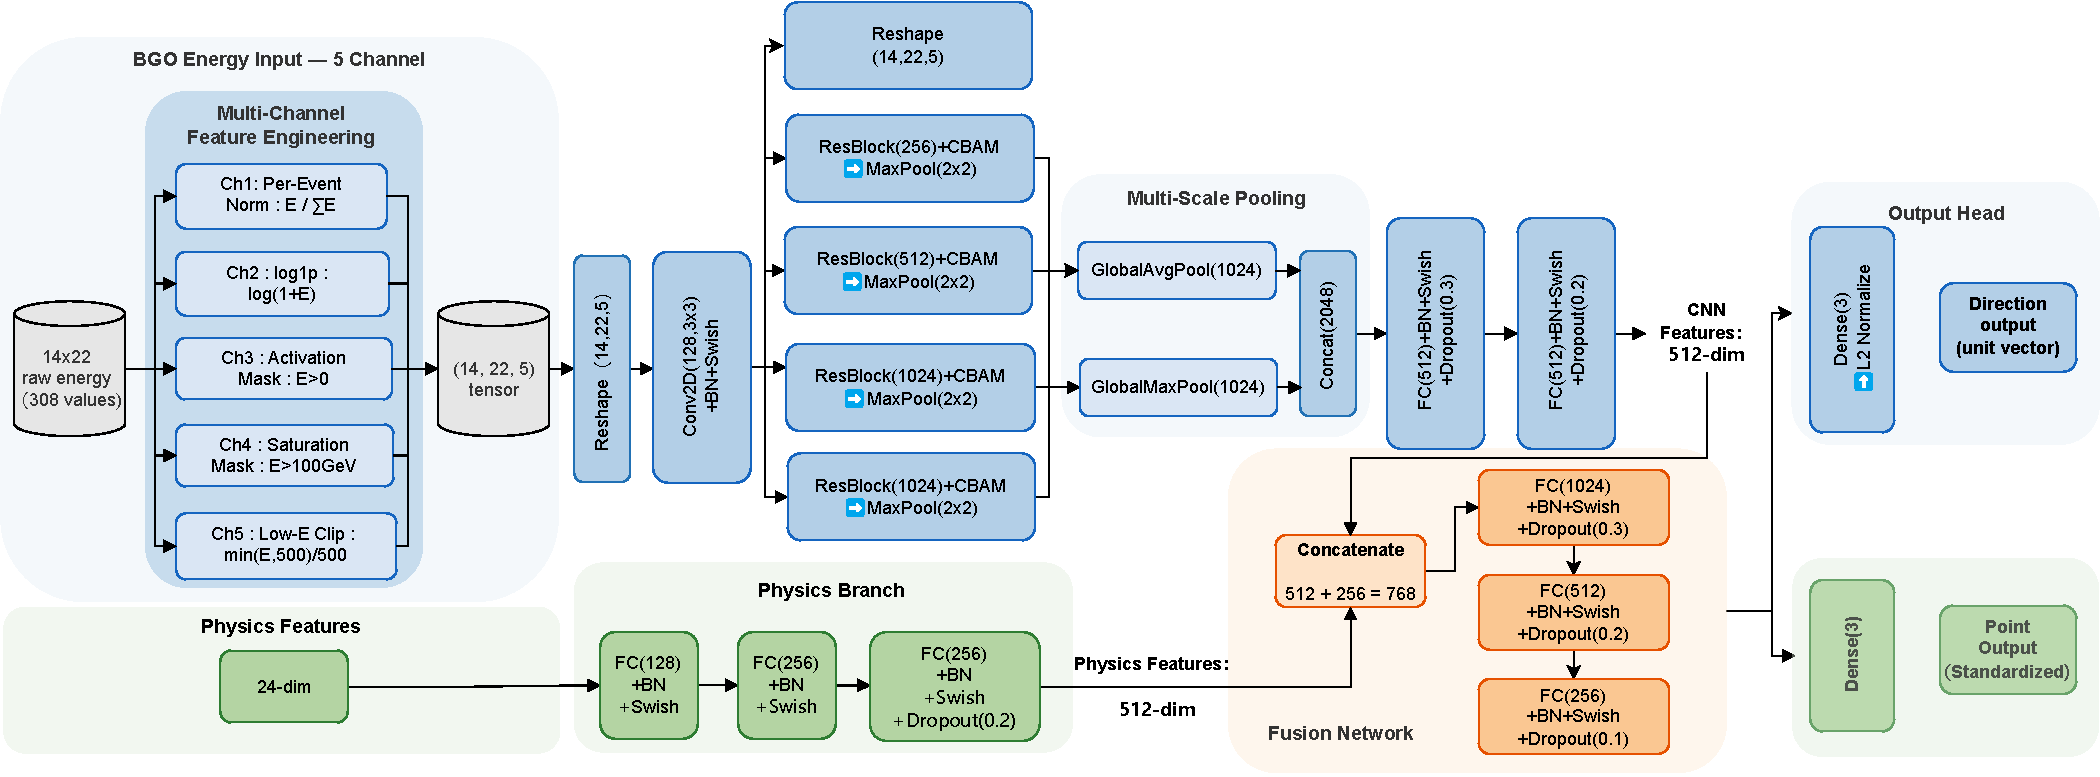
\includegraphics[width=1.0\textwidth]{graph/large_architecture.pdf}
\caption{Schematic overview of the Deep-Learning-Dominant (DLD) architecture for large-angle events ($60^{\circ}$--$90^{\circ}$). The model processes a 5-channel BGO energy input (per-event normalized energy, log-transformed energy, an activation mask, a saturation mask, and a low-energy clip) together with a 24-dimensional handcrafted physics feature vector, extracts features via a CNN backbone with residual blocks~\cite{he2016deep} and CBAM attention~\cite{woo2018cbam}, and jointly predicts direction and impact point through a multi-task fusion network.}
\label{fig:large_angle_reco}
\end{figure}

\textbf{Input Representation:} The DLD model consumes a 5-channel BGO energy map of shape $(14,22,5)$ together with a 24-dimensional handcrafted physics feature vector. The five energy channels are \textbf{(Ch1)} per-event normalized energy $E_{ij}/\sum E$, which captures the relative shower shape; \textbf{(Ch2)} log-transformed energy $\ln(1+E_{ij})$, which preserves low-energy peripheral detail and compresses the wide dynamic range of high-energy electrons; \textbf{(Ch3)} an activation mask $\mathbb{I}(E_{ij}>0)$ indicating deposition presence; \textbf{(Ch4)} a saturation mask $\mathbb{I}(E_{ij}>100\,\text{GeV})$ flagging bars whose energy exceeds an empirical threshold, chosen because TeV-scale electromagnetic showers frequently drive single-crystal digitiser channels toward saturation; and \textbf{(Ch5)} a low-energy clip $\min(E_{ij},500\,\text{MeV})/500$ that isolates peripheral shower topology by capping core deposits at an empirical 500\,MeV ceiling. In parallel, the physics stream receives a regime-specific 24-dimensional handcrafted vector (distinct from both the 7-dimensional morphology vector used by the Angle Classifier in Section~\ref{ssec:classifier} and the 24-dimensional standard-angle vector of Section~\ref{sec:data}); it contains, for each of the 7 layer pairs, the normalized Y-view energy, the normalized X-view energy, and the energy-weighted centroid of the Y-view bars, plus three global quantities: the logarithm of the total deposited energy, the active-bar fraction, and the index of the shower-maximum layer. These features encode geometric priors that complement the learned representations.

\textbf{Network Architecture:} The DLD model follows a similar dual-stream structure to the PGHNN but with important adaptations. The CNN backbone processes the 5-channel input through initial Conv2D layers (128 filters), followed by four residual blocks with Convolutional Block Attention Modules (CBAM) at increasing depths (256, 512, 1024, 1024 filters), each incorporating dropout for regularization. Multi-scale pooling combines GlobalAveragePooling and GlobalMaxPooling to capture broad spatial features. The physics stream processes the 24-dimensional feature vector through fully connected layers (128--256--256 neurons). The fusion network (1024--512--256 neurons) integrates both streams and feeds into two task-specific heads.

\textbf{Multi-Task Learning Framework:} The DLD architecture predicts direction and impact point jointly, in a single multi-task pass: \textbf{(1)} Direction output: a 3D unit vector representing the particle trajectory, L2-normalized to ensure $|\vec{D}|=1$; and \textbf{(2)} Point output: the impact point coordinates on the generation sphere of radius 1.38\,m (Section~\ref{sec:data}, adopted as the reference-sphere radius $R$), representing the true incident location from Monte Carlo simulation. The point prediction is standardized using training set statistics to ensure stable gradients.

\textbf{Impact-Point Regression Weighting:} Training the network to predict both direction and impact point simultaneously for large-angle events is challenging due to spatial information loss from side leakage. We therefore keep the impact-point head dormant at the start of training and anneal its loss weight only after the directional head has consolidated, following the curriculum-learning principle that harder sub-tasks should be introduced only after easier ones are mastered~\cite{bengio_2009}. Concretely, a \texttt{PointWeightAnnealing} schedule sets the point-loss weight to zero for the first 15 epochs and then ramps it linearly to a final value of $0.1$ over the subsequent 15 epochs, after which it is held fixed; the point loss itself is a Huber loss with $\delta=0.5$. This delayed, gradual introduction prevents the point-head gradient from disrupting the directional head during early training and avoids convergence to local minima caused by ambiguous impact points in leaking showers.

\textbf{Loss Function Design:} The DLD model employs a specialized loss function accounting for the specific challenges of large-angle reconstruction. Table~\ref{tab:loss_comparison} summarizes the key differences between the standard and large-angle models.

\begin{table}[htbp]
\centering
\caption{Comparison of loss function components between the PGHNN (standard-angle) and DLD (large-angle) models.}
\label{tab:loss_comparison}
\small
\setlength{\tabcolsep}{6pt}
\renewcommand{\arraystretch}{1.15}
\begin{tabular*}{\textwidth}{@{\extracolsep{\fill}}p{0.22\textwidth}p{0.36\textwidth}p{0.36\textwidth}}
\hline
\textbf{Component} & \textbf{Standard ($0^{\circ}$--$60^{\circ}$)} & \textbf{Large-Angle ($60^{\circ}$--$90^{\circ}$)} \\ \hline
Direction Loss & $0.1\mathcal{L}_{\text{MSE}} + 0.9(1{-}\cos\theta)^2$ & $0.1\mathcal{L}_{\text{MSE}} + 0.9(1{-}\cos\theta) + 0.05\mathcal{L}_{\text{flip}}$ \\
Flip Penalty & Not used & $\lambda\,\mathbb{I}(z_{\rm p}z_{\rm t}{<}0)$, $\lambda{=}0.05$ \\
Point Loss & $0.01\,\mathcal{L}_{\text{Huber},\delta=2.0}$ \newline (minimal weight) & $w_{\rm pt}(t)\,\mathcal{L}_{\text{Huber},\delta=0.5}$, \newline annealed $0{\to}0.1$ (ep.~15--30) \\ \hline
\end{tabular*}
\normalsize
\end{table}

The direction loss combines MSE ($\alpha=0.10$), the linear cosine term $1-\cos\theta$ ($\beta=0.90$), and a flip penalty ($\lambda=0.05$) that penalizes 180° directional reversals when $z_{\text{pred}}$ and $z_{\text{true}}$ have opposite signs. The impact-point head uses a Huber loss with $\delta=0.5$ whose weight $w_{\rm pt}(t)$ is annealed from $0$ to $0.1$ over training epochs 15–30.

\textbf{Hemisphere ambiguity.} A BGO-only reconstruction cannot, in principle, determine a priori whether a shower was initiated by a downward-going particle entering from above the detector or an upward-going particle entering from below, because the calorimeter records only energy deposition and not the absolute direction of incidence. The flip penalty above resolves this at training time by enforcing consistency with the Monte Carlo truth: it penalizes predictions whose $z$-component has the opposite sign to the true direction ($z_{\text{pred}}\cdot z_{\text{true}}<0$), so the network learns to orient the predicted vector according to the true incident hemisphere of the training sample. Because the training data in this work are downward-going events ($0^{\circ}\le\theta\le 90^{\circ}$), the model implicitly adopts the downward convention, and at inference it assumes downward incidence, a valid assumption for the validated $0^{\circ}$--$90^{\circ}$ range. Consequently, any residual hemisphere mis-assignment is expected to be negligible for the validated downward-going $0^{\circ}$--$90^{\circ}$ sample; correctly resolving upward-going events in the future $90^{\circ}$--$130^{\circ}$ extension will require either an explicit hemisphere classifier or the use of the earliest shower-development layer as a directional prior.


\FloatBarrier

\subsection{Training Protocol and Implementation Details}
\label{ssec:training}

For reproducibility we summarize the training configuration of the two expert models; both share the backbone described in Sections~\ref{ssec:standard} and~\ref{ssec:large} and are trained independently on overlapping but not identical angular sub-ranges.

\textbf{Optimizer and learning-rate schedule.} The two models use different schedules. The standard-angle model is optimized with Adam using a \texttt{CyclicalLearningRate} schedule ($\mathrm{base\_lr}=10^{-5}$, $\mathrm{max\_lr}=8\times10^{-4}$, $\mathrm{step\_size}=2500$; $\mathrm{clipnorm}=1.0$; default $\beta_{1}=0.9$, $\beta_{2}=0.999$, $\epsilon=10^{-7}$). The large-angle model is optimized with Adam ($\mathrm{clipnorm}=1.0$) using a \texttt{CyclicalLearningRate} schedule ($\mathrm{base\_lr}=10^{-5}$, $\mathrm{max\_lr}=8\times10^{-4}$, $\mathrm{step\_size}=2500$) preceded by a linear warm-up of 3000 steps from an initial rate of $2\times10^{-5}$ (\texttt{WarmupLR}).

\textbf{Batch size and epochs.} Both models are trained with batch size 2048 for up to 200 epochs each (with early stopping, patience 20, monitoring the validation angular error; training typically converges well before the nominal maximum).

\textbf{Losses.} The composite losses are those defined in Sections~\ref{ssec:standard} and~\ref{ssec:large}. The standard-angle model combines an MSE term ($\alpha=0.1$), the squared cosine term $(1-\cos\theta)^2$ ($\beta=0.9$), and a small impact-point Huber term ($w_{\rm pt}=0.01$, $\mathcal{L}_{\text{Huber},\delta=2.0}$); it \emph{does} output an impact-point head, whose weight is intentionally negligible so that direction regression dominates. The large-angle model additionally includes a flip penalty and an impact-point Huber loss ($\delta=0.5$) whose weight is annealed from $0$ to $0.1$ over epochs 15–30.

\textbf{Data scale and split.} Training uses the Monte Carlo samples of Section~\ref{sec:data}: of the $11{,}894{,}154$ events spanning $100$~GeV--$1$~TeV and zenith range $0^{\circ}$--$90^{\circ}$, the $80\%$ training partition ($9{,}515{,}323$ events) is used for model training and the remaining $20\%$ for evaluation, stratified by $(\theta,E)$.

\textbf{Training angular support.} The standard-angle PGHNN is trained on
events in $0^{\circ}$--$70^{\circ}$ and the large-angle DLD on events in
$50^{\circ}$--$90^{\circ}$, so both models see showers from either side of
the $60^{\circ}$ routing threshold. The SVM still routes events at
$60^{\circ}$; extending the training ranges does not change this rule.

\textbf{Hardware and inference cost.} All models were trained on a single NVIDIA A100 (80\,GB) GPU with CUDA 11.7, cuDNN 8.6.0.163, TensorFlow 2.10, and Python 3.10. A single event is reconstructed in approximately $1.5$\,ms on the same GPU, and a full training run requires approximately $20$~h; these figures confirm that the method is feasible for offline ground processing of the DAMPE downlink stream.

\FloatBarrier
\section{Performance Evaluation}
\label{sec:eval}

\subsection{Evaluation Metrics}

The quality of the trajectory reconstruction is quantified using three primary metrics: \textbf{Angular Resolution ($\Psi_{68}$), Cosine Similarity, and Reconstruction Efficiency.}

Angular Resolution ($\Psi_{68}$) is defined as the space angle containing 68\% of the reconstructed events relative to the true MC truth direction. The space angle error $\psi$ for a single event is calculated as:
\begin{equation}
\psi = \arccos(\hat{\mathbf{v}}_{\text{pred}} \cdot \hat{\mathbf{v}}_{\text{true}})
\end{equation}
where $\hat{\mathbf{v}}_{\text{pred}}$ and $\hat{\mathbf{v}}_{\text{true}}$ are the unit vectors of the predicted and true particle directions, respectively. The metric $\Psi_{68}$ represents the 68th percentile of the distribution of $\psi$.

Cosine Similarity measures the alignment accuracy between the predicted and true vectors, providing a direct metric for directional coherence:
\begin{equation}
\text{Cosine Similarity} = \frac{\mathbf{v}_{\text{pred}} \cdot \mathbf{v}_{\text{true}}}{\|\mathbf{v}_{\text{pred}}\| \|\mathbf{v}_{\text{true}}\|}
\end{equation}
Values closer to 1.0 indicate higher reconstruction accuracy.

Reconstruction Efficiency evaluates the robustness of the algorithm. It is defined as the fraction of the events entering the evaluation that are reconstructed with an angular error below a tolerance threshold of $10^{\circ}$:
\begin{equation}
\epsilon = \frac{N(\psi < 10^{\circ})}{N_{\text{total}}}
\end{equation}
where $N_{\text{total}}$ is the number of simulated events in the evaluation sample. The same denominator is used for every method compared in this work, so that the efficiencies are directly comparable, and no trigger-efficiency correction is applied. Events with $\psi \ge 10^{\circ}$ are counted as reconstruction failures.

In addition to the directional metrics above, we introduce the Arc-Length Error to evaluate the impact point reconstruction precision of the two expert models. Both models predict the incident point at the generation sphere of Section~\ref{sec:data} (radius 1.38\,m), so the reconstructed trajectory is the straight line that passes through the predicted impact point $\vec{P}_{\text{pred}}$ along the predicted direction $\hat{\mathbf{v}}_{\text{pred}}$. The Arc-Length Error is defined as the great-circle distance on the reference sphere between the true incident point and the upstream (entrance-side) intersection of this line with the same sphere. Let $\hat{\mathbf{u}}_{\text{true}}$ and $\hat{\mathbf{u}}_{\text{pred}}$ denote the unit vectors from the sphere center to the true point and to that intersection, respectively. The arc-length error $s$ is given by:
\begin{equation}
s = R \cdot \arccos(\hat{\mathbf{u}}_{\text{true}} \cdot \hat{\mathbf{u}}_{\text{pred}})
\end{equation}
where $R$ is the reference-sphere radius, taken to be the generation radius of 1.38\,m. The vector $\hat{\mathbf{u}}_{\text{pred}}$ therefore points to where the reconstructed line crosses the entrance surface, which is the incident position a downstream analysis would use. Because the predicted impact point is confined to a thin shell around the reference sphere, this intersection is dominated by the tangential position of $\vec{P}_{\text{pred}}$ and is only weakly sensitive to $\hat{\mathbf{v}}_{\text{pred}}$ (Section~\ref{sec:eval}); $s$ is thus a measure of the entry-point displacement, that is, of the impact-point prediction, and not a restatement of the angular resolution.

\subsection{Reconstruction Efficiency and Accuracy}
\label{ssec:efficiency}

A major limitation of the Standard BGO Algorithm is the loss of usable events at large incidence angles. Table~\ref{tab:efficiency} shows that its efficiency, defined by the $\psi<10^{\circ}$ criterion of Section~\ref{sec:eval}, is $98.73\%$ in $0^{\circ}$--$30^{\circ}$ and $91.06\%$ in $30^{\circ}$--$60^{\circ}$, but falls to $38.58\%$ in $60^{\circ}$--$90^{\circ}$. Combined with the angular resolution of $\Psi_{68}=32.73^{\circ}$ in that band (Table~\ref{tab:accuracy}), this means that the majority of large-angle events are still reconstructed with unusable directions. The degradation follows from the failure of the shower axis fit when the shower maximum leaks out of the calorimeter. In contrast, the PGHNN and DLD framework achieves near 100\% efficiency across the entire $0^{\circ}$--$90^{\circ}$ domain, thereby extending the detector field of view.

\begin{table}[htbp]
    \centering
    \caption{Comparison of Reconstruction Efficiency across different angular ranges.}
    \label{tab:efficiency}
    \begin{tabular*}{\textwidth}{@{\extracolsep{\fill}}lccc}
    \hline
    \textbf{Method} & \textbf{0$^{\circ}$--30$^{\circ}$} & \textbf{30$^{\circ}$--60$^{\circ}$} & \textbf{60$^{\circ}$--90$^{\circ}$} \\ \hline
    Standard BGO Algorithm & 98.73\% & 91.06\% & 38.58\% \\ 
    PGHNN (This work) & \textbf{100\%} & \textbf{99.47\%} & \textbf{----} \\
    DLD (This work) & \textbf{----} & \textbf{----} & \textbf{99.50\%} \\ \hline
    \end{tabular*}
\end{table}

Table~\ref{tab:accuracy} compares the angular resolution ($\Psi_{68}$) of the methods. In the standard-angle region ($0^{\circ}$--$60^{\circ}$), the PGHNN reduces $\Psi_{68}$ from $3.78^{\circ}$ to $1.40^{\circ}$ (a factor of $\approx 2.7$) by combining physical priors with the dynamic fusion mechanism. In the large-angle region ($60^{\circ}$--$90^{\circ}$), the Standard BGO Algorithm degrades to $\Psi_{68}=32.73^{\circ}$ (with a reconstruction efficiency of $38.58\%$ under the $\psi<10^{\circ}$ criterion of Section~\ref{sec:eval}), whereas the DLD maintains $1.31^{\circ}$ (a factor of $\approx 25$).

\begin{table}[htbp]
    \centering
    \caption{Comparison of Angular Resolution ($\Psi_{68}$, lower is better).
    The Standard BGO Algorithm entries are obtained with the official DAMPE
    energy-weighted CoG track reconstruction applied to the same Monte Carlo
    electron sample as the two deep-learning models. The conventional BGO+STK
    pipeline is listed for reference only: quoted at
    10~GeV from Ref.~\cite{dampe_stk_perf}, it operates within
    $0^{\circ}$--$60^{\circ}$ and is not evaluated on the 100~GeV--1~TeV sample
    used here; it is therefore not directly comparable to the BGO-only methods
    in the same energy band.}
    \label{tab:accuracy}
    \begin{tabular*}{\textwidth}{@{\extracolsep{\fill}}lc}
    \hline
    \textbf{Method} & \textbf{68\% Quantile (degree)} \\ \hline
    Conventional BGO+STK pipeline ($0^{\circ}$--$60^{\circ}$) & \textbf{0.2} \\
    Standard BGO Algorithm ($0^{\circ}$--$60^{\circ}$) & 3.78 \\ 
    Standard BGO Algorithm ($60^{\circ}$--$90^{\circ}$) & 32.73 \\
    PGHNN Method ($0^{\circ}$--$60^{\circ}$) & 1.40 \\
    DLD Method ($60^{\circ}$--$90^{\circ}$) & \textbf{1.31} \\ \hline
    \end{tabular*}
    \end{table}

Figure~\ref{fig:angle_residuals} presents the direction residual distributions for both angular regimes. In the standard-angle regime (top panel), the zenith and azimuth residuals exhibit approximately symmetric, unimodal distributions centered near zero, with the space angle error distribution peaking at approximately $0.8^{\circ}$. The large-angle regime (bottom panel) shows a similar overall shape but with a modestly broader width, particularly in the azimuth residual and space angle error, reflecting the increased reconstruction challenge posed by shower leakage. Both distributions are centered near zero with negligible mean offset, confirming the high accuracy of the reconstructed directions.

\begin{figure}[htbp]
    \centering
    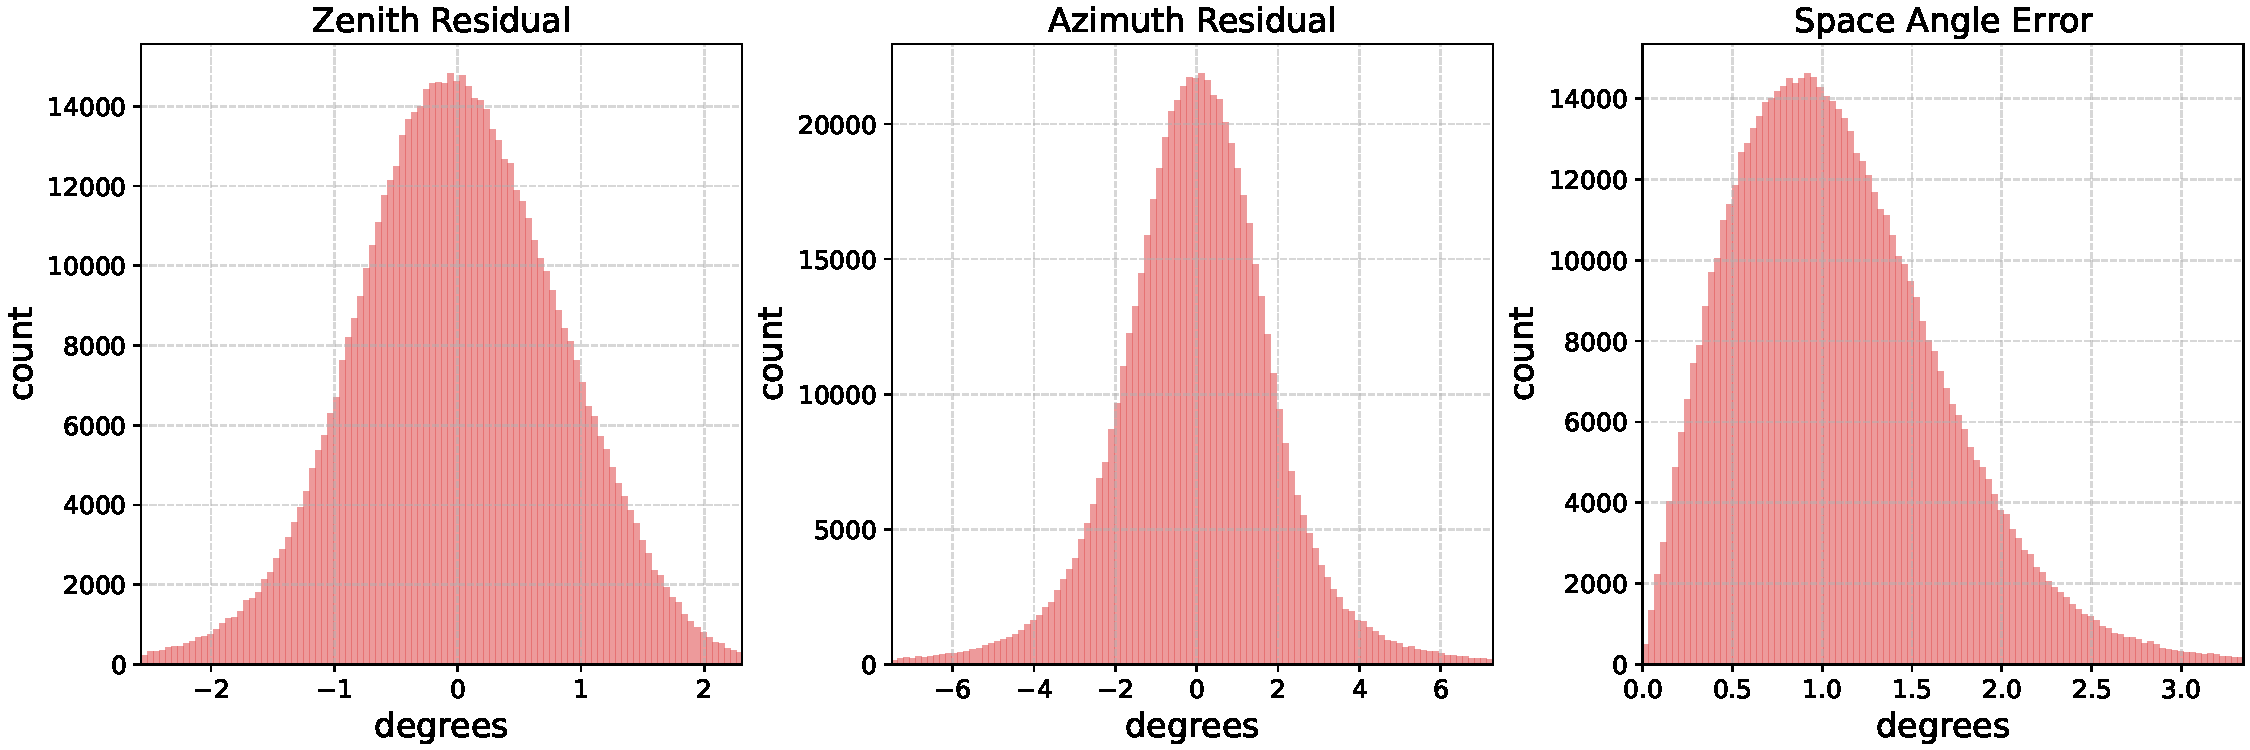
\includegraphics[width=0.9\textwidth]{graph_update/angle_only_hist_0_60.pdf}
    
    \vspace{0.3cm}
    
    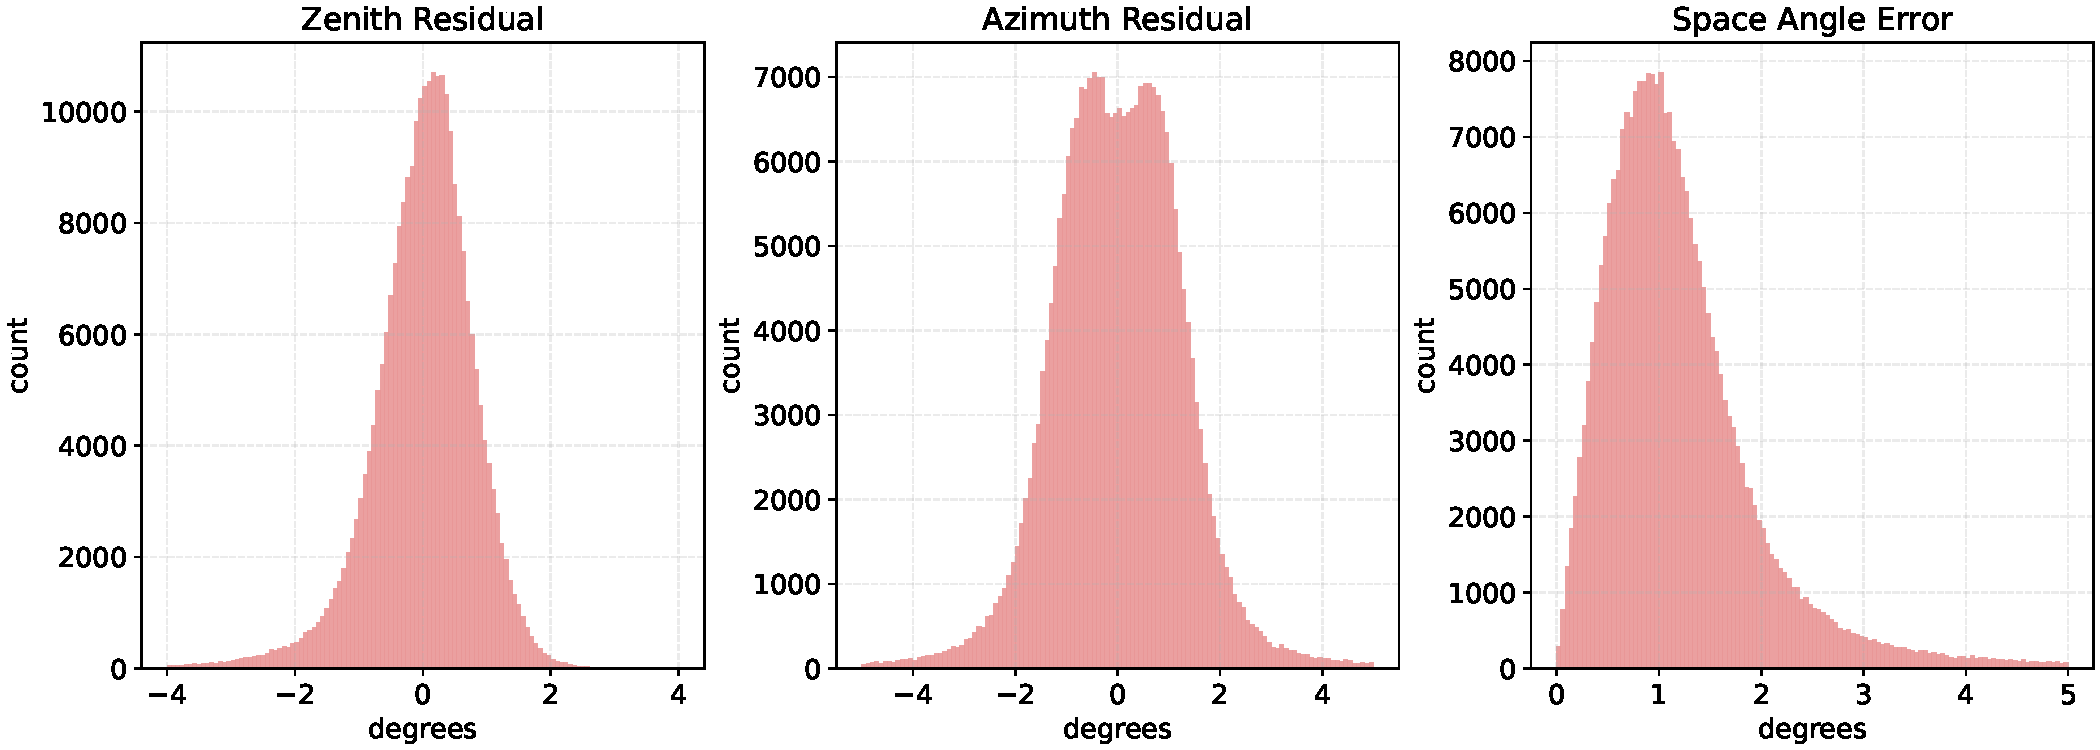
\includegraphics[width=0.9\textwidth]{graph_update/angle_only_hist_60_90.pdf}
    \caption{Direction residual distributions for the standard-angle regime (top, PGHNN) and the large-angle regime (bottom, DLD). Within each panel (left to right): zenith residual, azimuth residual, and space angle error.}
    \label{fig:angle_residuals}
\end{figure}

\subsection{Energy Dependence and Stability}

The performance stability across primary particle energies is evaluated in Figure~\ref{fig:resolution_energy}. The Standard BGO Algorithm (black dashed line), evaluated on the same Monte Carlo sample in the $0^{\circ}$--$60^{\circ}$ range, shows a mild energy dependence: $\Psi_{68}$ is approximately $4.0^{\circ}$ at 100~GeV, rises slightly to $\sim 4.05^{\circ}$ around 150~GeV, and then decreases steadily to $\sim 3.5^{\circ}$ towards 1~TeV. The energy-integrated value of $3.78^{\circ}$ quoted in Table~\ref{tab:accuracy} is consistent with these per-bin values. Such behaviour is characteristic of conventional calorimetric methods, whose precision is limited by the statistics of the energy deposition. In contrast, the PGHNN (red) and DLD (blue) curves change much less with energy than the standard algorithm, improving slightly from $\sim 1.5^{\circ}$ and $\sim 1.4^{\circ}$ to $\sim 1.3^{\circ}$ and $\sim 1.2^{\circ}$, respectively. This mild energy response suggests that the physics-guided PGHNN extracts topological features of the shower axis that are less sensitive to energy scale, compensating for the fluctuations that limit analytical approaches at lower energies.

\begin{figure}[htbp]
    \centering
    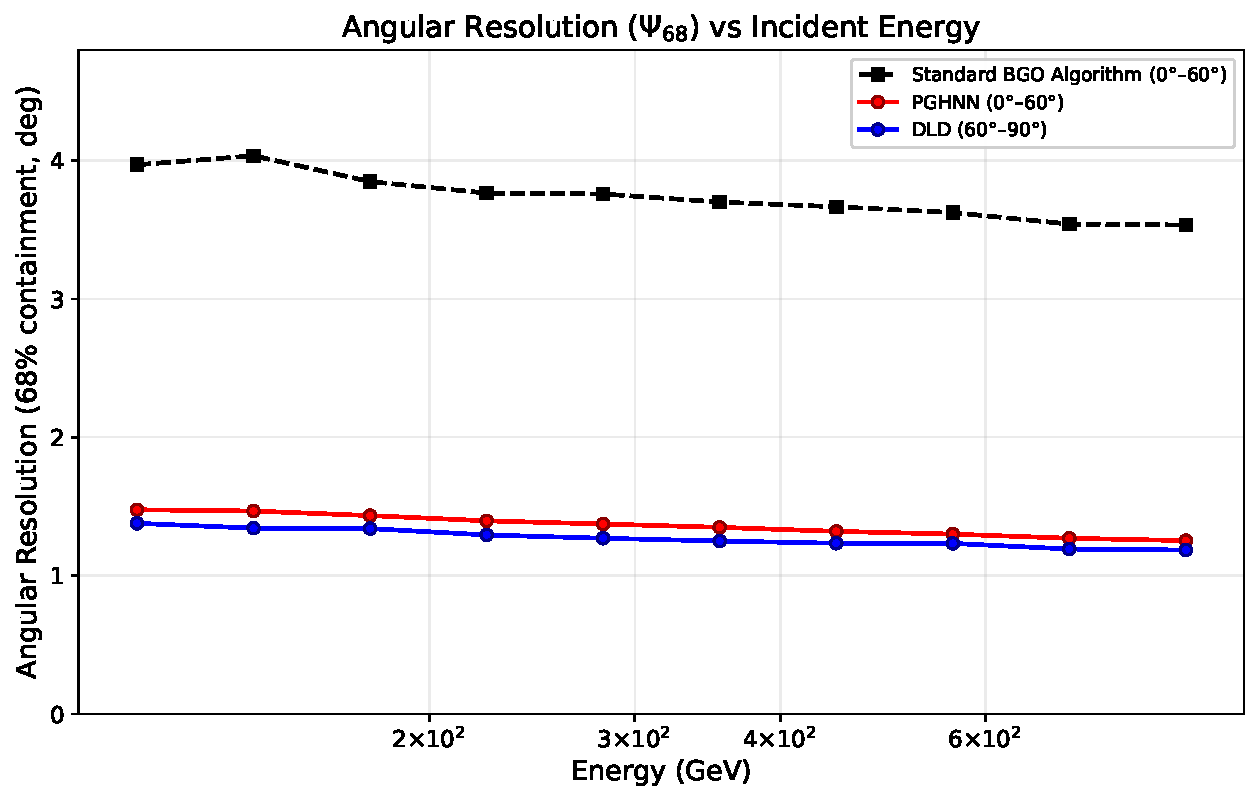
\includegraphics[width=0.8\textwidth]{graph_update/merged_angular_resolution_vs_energy.pdf}
    \caption{Angular resolution ($\Psi_{68}$) versus incident energy over the
    100~GeV--1~TeV range, comparing the Standard BGO Algorithm (black dashed, $0^{\circ}$--$60^{\circ}$),
    the PGHNN ($0^{\circ}$--$60^{\circ}$, red) and the DLD
    ($60^{\circ}$--$90^{\circ}$, blue). The energy-integrated $\Psi_{68}$ of the
    Standard BGO Algorithm is $3.78^{\circ}$
    (Table~\ref{tab:accuracy}).}
    \label{fig:resolution_energy}
\end{figure}

For the large-angle regime ($60^{\circ}$--$90^{\circ}$), the DLD model exhibits a systematic energy dependence, as shown by the blue curve in Figure~\ref{fig:resolution_energy}. Across the 100~GeV to ${\sim}900~\mathrm{GeV}$ range, the angular resolution improves monotonically from approximately $1.4^{\circ}$ to $1.2^{\circ}$. While this energy dependence is more pronounced than that of the PGHNN in the standard-angle regime, the absolute resolution remains well below $1.5^{\circ}$ across the entire range. This behavior indicates that the five-channel input representation and the curriculum learning strategy enable the network to extract directional features even when a substantial fraction of the shower energy escapes the calorimeter.

\subsection{Impact Point Reconstruction Precision}

In addition to directional accuracy, the joint prediction of the incident point by the DLD model enables a direct assessment of impact point reconstruction precision via the Arc-Length Error metric defined in Section~\ref{sec:eval}. Figure~\ref{fig:arc_error_hist} presents the distributions of arc-length errors for both angular regimes overlaid as normalized probability densities. In the standard-angle range ($0^{\circ}$--$60^{\circ}$), the arc-length error achieves a P68 of 32.99~mm and a P95 of 55.17~mm, corresponding to an angular deviation of approximately $1.37^{\circ}$ and $2.29^{\circ}$ on the reference sphere, respectively. For the large-angle regime ($60^{\circ}$--$90^{\circ}$), where side leakage complicates both direction and impact point estimation, the arc-length error achieves a P68 of 38.48~mm and a P95 of 80.99~mm, equivalent to angular deviations of approximately $1.60^{\circ}$ and $3.36^{\circ}$, respectively. The two distributions differ chiefly in their tail behaviour: the standard-angle distribution decays rapidly beyond $\sim 55$~mm, whereas the large-angle distribution exhibits a noticeably heavier tail extending beyond $\sim 100$~mm, reflecting the increased challenge of impact-point reconstruction under grazing-incidence geometry.

\begin{figure}[htbp]
    \centering
    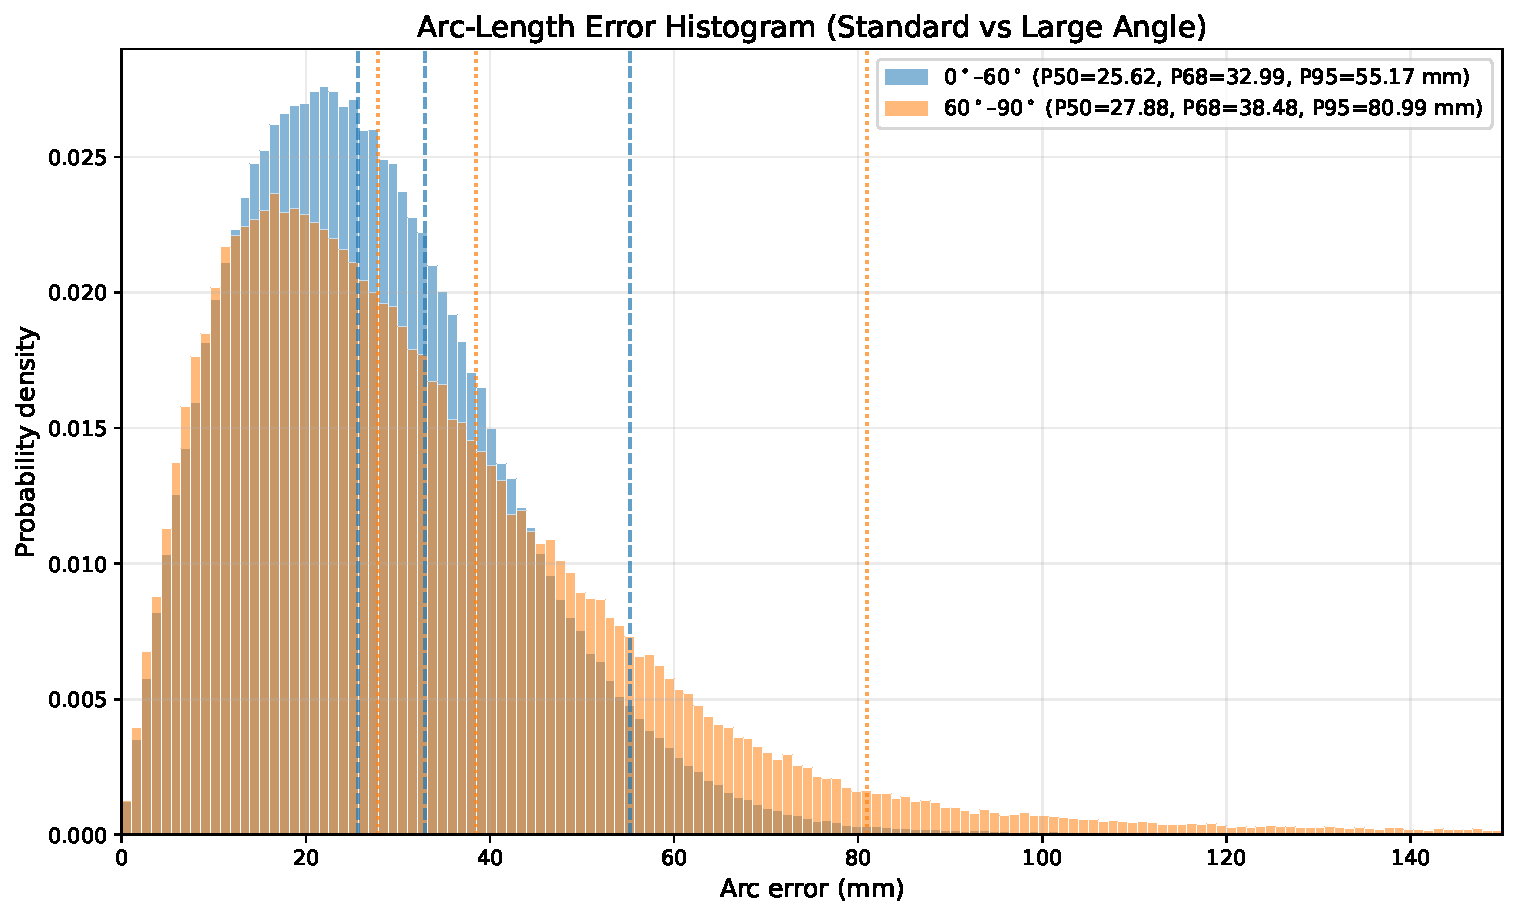
\includegraphics[width=0.85\textwidth]{graph_update/combined_arc_error_hist.pdf}
    \caption{Arc-length error distributions for the standard-angle regime (blue, $0^{\circ}$--$60^{\circ}$) and the large-angle regime (orange, $60^{\circ}$--$90^{\circ}$), overlaid as normalized probability densities. Vertical lines in same color mark the P50, P68 and P95 percentiles of each distribution.}
    \label{fig:arc_error_hist}
\end{figure}

To investigate the angular dependence of the impact point precision, Figure~\ref{fig:arc_error_boxplot} shows the arc-length error statistics binned by equal-area intervals in $\cos\theta$. In the standard-angle regime, the P68 values are approximately 37~mm for the 0$^{\circ}$--33.6$^{\circ}$ bin, 25~mm for the 33.6$^{\circ}$--48.2$^{\circ}$ bin, and 36~mm for the 48.2$^{\circ}$--60$^{\circ}$ bin. In the large-angle regime, the P68 values are approximately 38~mm for the 60$^{\circ}$--70.5$^{\circ}$ bin, 38~mm for the 70.5$^{\circ}$--80.4$^{\circ}$ bin, and 41~mm for the 80.4$^{\circ}$--90$^{\circ}$ bin. The P95 values remain below 100~mm across all bins, confirming that the multi-task learning framework maintains acceptable impact point precision even under extreme leakage conditions.

\begin{figure}[htbp]
    \centering
    \begin{subfigure}{\textwidth}
        \centering
        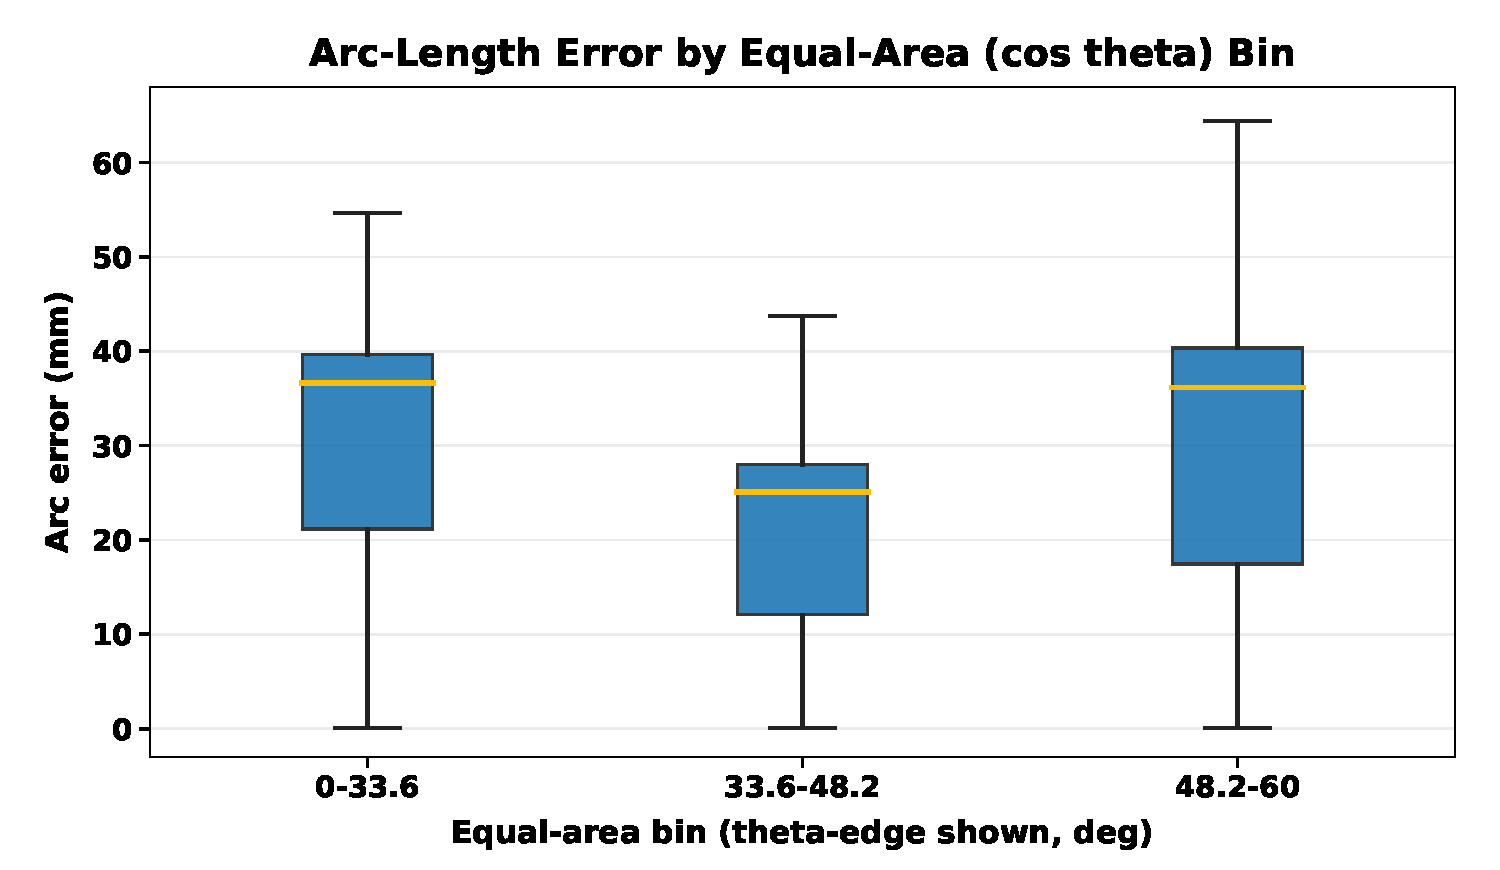
\includegraphics[width=0.65\textwidth]{graph_update/arc_error_cos_boxplot_0_60.pdf}
        \caption{Standard-angle regime ($0^{\circ}$--$60^{\circ}$).}
        \label{fig:arc_error_boxplot_standard}
    \end{subfigure}
    \\[6pt]
    \begin{subfigure}{\textwidth}
        \centering
        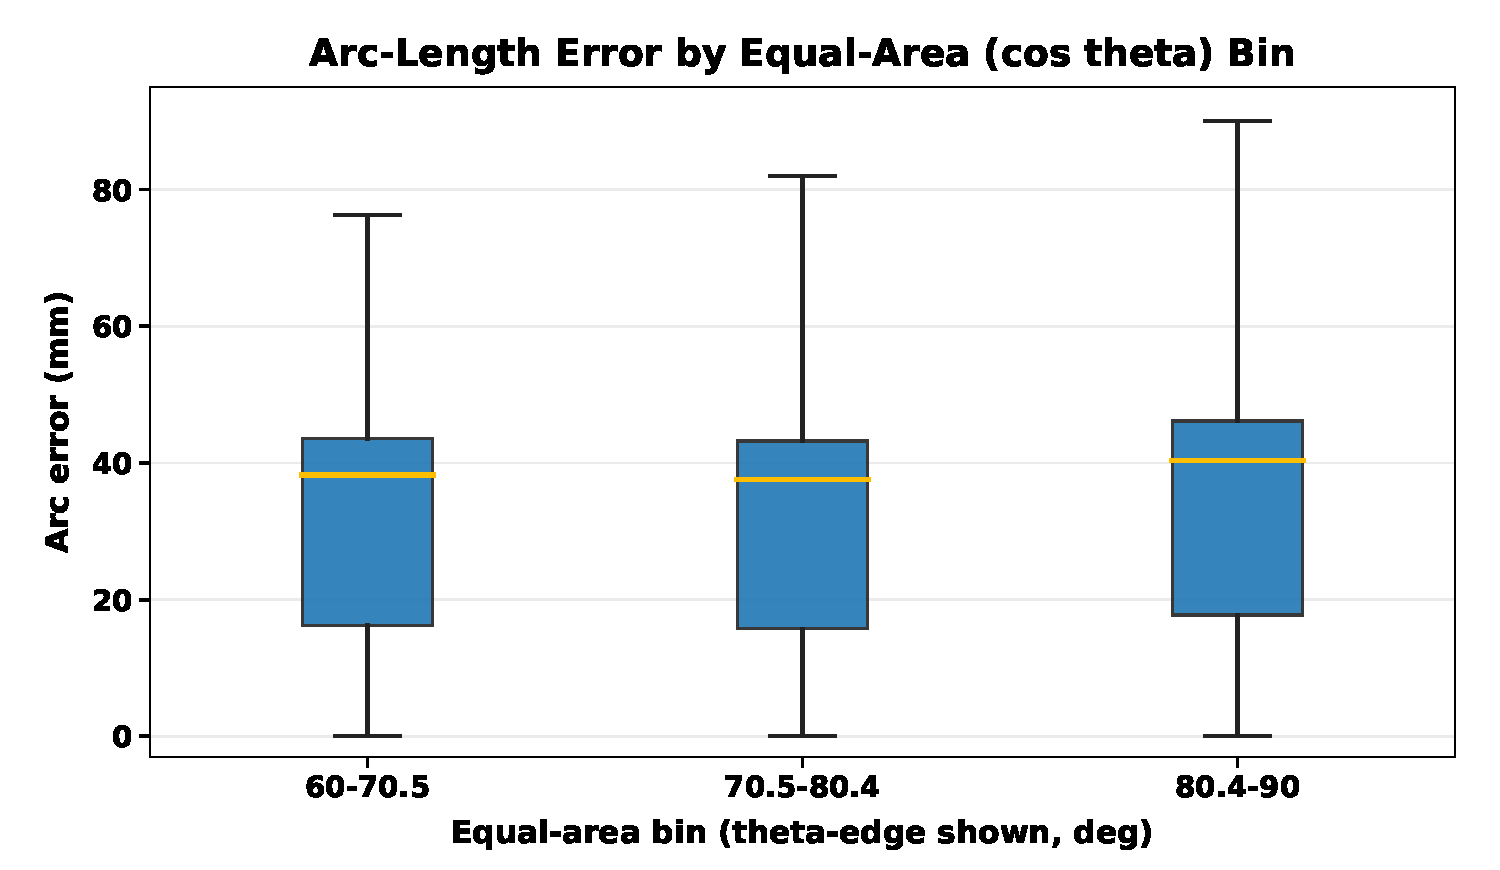
\includegraphics[width=0.65\textwidth]{graph_update/arc_error_cos_boxplot_60_90.pdf}
        \caption{Large-angle regime ($60^{\circ}$--$90^{\circ}$).}
        \label{fig:arc_error_boxplot_large}
    \end{subfigure}
    \caption{Arc-length error statistics by equal-area $\cos\theta$ bins for (a) the standard-angle regime and (b) the large-angle regime. The box spans Q1--Q3, the yellow line marks P68, and the whiskers extend to the minimum and P95.}
    \label{fig:arc_error_boxplot}
\end{figure}

The arc-length error is not a second measurement of the direction: it records where the reconstructed line crosses the entrance sphere. The predicted impact point lies close to that sphere, so the reconstructed line meets it close to $\vec{P}_{\text{pred}}$; only the residual radial offset of the prediction acts as a lever arm for the directional error, and for the resolutions reported here ($\sim1.3^{\circ}$--$1.4^{\circ}$) it contributes well under a millimetre. The arc-length error is therefore a measure of the tangential accuracy of the impact-point prediction, and the two regimes can be compared directly: the entry point is located to $3.3$\,cm (P68) at standard angles and $3.8$\,cm at large angles, a degradation of only about $17\%$ where the shower is truncated by side leakage. The ability to reconstruct the incident point with centimeter-level precision (P68 $<$ 5~cm) is scientifically valuable, as it enables the extension of particle identification algorithms (particularly electron--hadron discrimination) into the large-angle regime~\cite{ambrosi_2017}, where the shower morphology relative to the precise axis is a relevant input to rejection variables.

\subsection{Boundary Analysis and Transition Strategy}
\label{ssec:boundary}

A hierarchical pipeline that routes events with a hard threshold at
$60^{\circ}$ is intrinsically sensitive to how the two expert models behave
at that boundary. If each expert is trained only on its own, disjoint angular
domain, neither network has seen showers from the other side of the
threshold; events close to $60^{\circ}$ are then reconstructed by a model
operating at the edge of its training support, and the routed angular
resolution can change abruptly when the classifier switches branches. We
therefore examine the continuity of $\Psi_{68}$ across the routing threshold
and describe a training-domain overlap that removes this discontinuity.

The routing rule is unchanged: the SVM classifier of
Section~\ref{ssec:classifier} assigns $0^{\circ}$--$60^{\circ}$ events to the
PGHNN and $60^{\circ}$--$90^{\circ}$ events to the DLD, and inference remains
a single hard routing decision. We extend only the angular support of the
training samples. The standard-angle model is trained on events spanning
$0^{\circ}$--$70^{\circ}$ instead of $0^{\circ}$--$60^{\circ}$, and the
large-angle model on $50^{\circ}$--$90^{\circ}$ instead of
$60^{\circ}$--$90^{\circ}$ (Section~\ref{ssec:training}). Each expert thus
sees a $10^{\circ}$ overlap band straddling the nominal boundary, while the
overall Monte Carlo sample of Section~\ref{sec:data} is unchanged.

Figure~\ref{fig:boundary} shows the resulting stitched $\Psi_{68}$ curve over
$0^{\circ}$--$90^{\circ}$, where each branch is evaluated only in the angular
interval to which it is routed. The two branches now join continuously at
$60^{\circ}$: both give $\Psi_{68}\approx 1.2^{\circ}$--$1.3^{\circ}$ at the
boundary, and the step present when the models were trained on disjoint
domains is no longer visible. The resolution stays below $\sim 1.7^{\circ}$
over the full range: it rises from $\sim 0.8^{\circ}$ at small zenith angles
to $\sim 1.5^{\circ}$ near $35^{\circ}$, passes through a shallow local
minimum of $\sim 1.1^{\circ}$ near $63^{\circ}$, and shows a broad local
maximum of $\sim 1.7^{\circ}$ near $79^{\circ}$ before falling back to
$\sim 1.3^{\circ}$ at $90^{\circ}$. No extrapolation beyond the training
support of either model is shown in this figure.

The choice of $60^{\circ}$ rests on the two mechanisms identified in
Section~\ref{ssec:framework}---the STK fiducial-volume cutoff and the
degradation of the Standard BGO Algorithm, which coincide at this
angle---together
with the continuity of the routed resolution at that angle. The overlap
band regularizes the boundary during training: both experts have been
trained on showers from either side of the threshold, so the residual
misclassifications of the SVM, which are concentrated near $60^{\circ}$
(Section~\ref{ssec:classifier}), no longer produce a localized degradation
in resolution. The two predictions are not blended at inference time. A
continuous soft-transition scheme, in which the two predictions are
interpolated across the overlap band, is left for future work.

\begin{figure}[htbp]
    \centering
    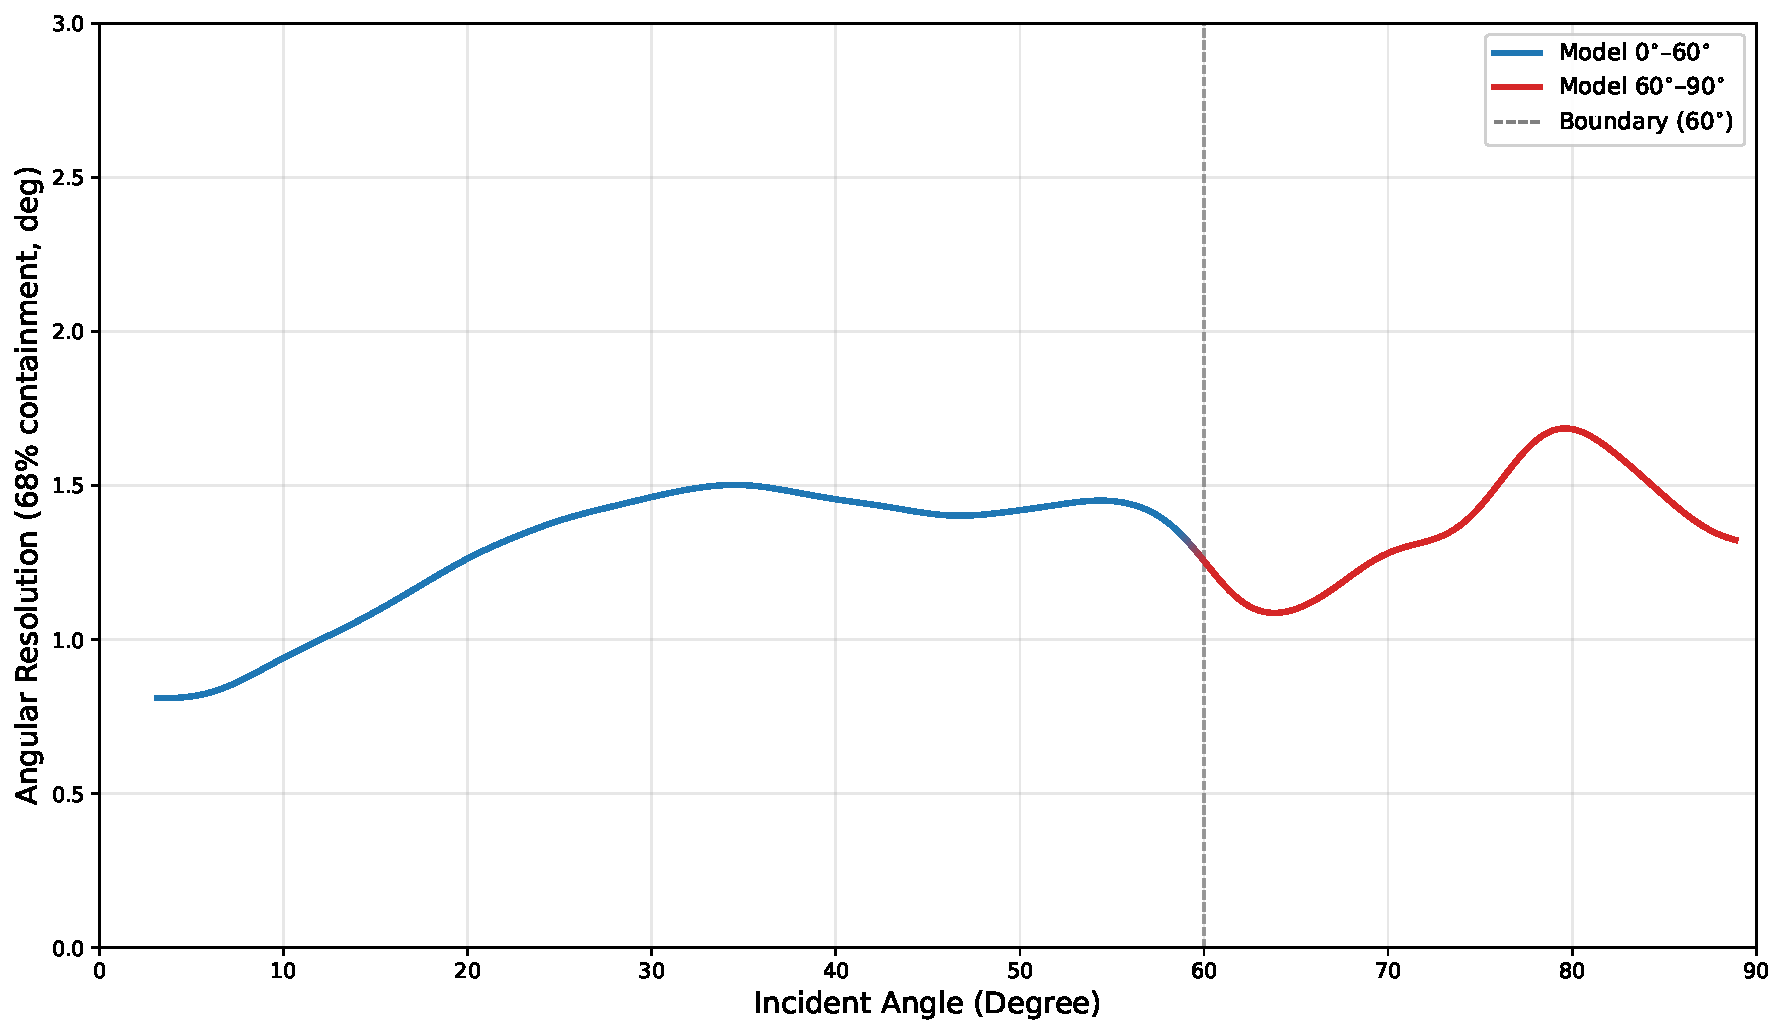
\includegraphics[width=0.85\textwidth]{graph_update/angular_resolution_stitched.pdf}
    \caption{Routed angular resolution ($\Psi_{68}$) versus incident angle
    across $0^{\circ}$--$90^{\circ}$ for the PGHNN (blue, labelled
    ``Model $0^{\circ}$--$60^{\circ}$'') and the DLD (red, labelled
    ``Model $60^{\circ}$--$90^{\circ}$''), each evaluated in the interval to
    which it is routed. Both models were trained on overlapping angular
    ranges ($0^{\circ}$--$70^{\circ}$ and $50^{\circ}$--$90^{\circ}$), so the
    two branches join continuously at the routing threshold. The vertical
    dashed line marks the $60^{\circ}$ boundary.}
    \label{fig:boundary}
\end{figure}


\FloatBarrier

\subsection{Ablation Study}
\label{ssec:ablation}

To substantiate the claim that the physics-guided components, rather than the deep-learning capacity alone, drive the reported accuracy, we perform an ablation study on the standard-angle (PGHNN) model, measuring the angular resolution $\Psi_{68}$ under each modification. The results are summarized in Table~\ref{tab:ablation}.

\begin{table}[htbp]
\centering
\caption{Ablation study on the standard-angle PGHNN model. $\Psi_{68}$ (degree, lower is better) is reported for the full model and for each modification.}
\label{tab:ablation}
\begin{tabular*}{\textwidth}{@{\extracolsep{\fill}}lc}
\hline
\textbf{Configuration} & \textbf{$\Psi_{68}$ (deg)} \\ \hline
Full PGHNN (24 physics features + dynamic fusion) & 1.40 \\
-- without the 24 physics features (energy-map only) & 1.81 \\
-- without dynamic fusion (always trust DL, $I_{\text{valid}}\equiv 0$) & 1.56 \\
-- reduced input (single channel) & 1.49 \\ \hline
\end{tabular*}
\end{table}

Removing the hand-crafted physics features degrades the resolution by $0.41^{\circ}$ (from $1.40^{\circ}$ to $1.81^{\circ}$), confirming that the feature engineering supplies geometric priors that the convolutional backbone alone exploits only partially. Disabling the physics-guided dynamic fusion (forcing the prediction to the deep-learning stream) yields a $0.16^{\circ}$ change ($1.56^{\circ}$ vs $1.40^{\circ}$), indicating that the arbitration between the analytical and data-driven branches contributes modestly but consistently. Reducing the input to a single channel provides a $0.09^{\circ}$ degradation ($1.49^{\circ}$ vs $1.40^{\circ}$), confirming the value of the dual-channel representation. Collectively, these ablations demonstrate that the improvements arise from concrete, separable components (physics-informed feature engineering, dynamic physics-guided fusion, and dual-channel input) within a measurable ``gray-box'' framework, rather than from an opaque black-box model; each contribution is measured, not merely asserted.

\FloatBarrier
\section{Discussion}
\label{sec:discussion}

\subsection{Application to Flight Data}
\label{ssec:flight}

The transition from Monte Carlo simulations to on-orbit flight data is
complicated by the absence of ground-truth incident-angle labels. The SVM
classifier of Section~\ref{ssec:classifier} addresses this by routing events
from shower morphology alone. As a first check on real detector data, we
apply the resulting pipeline to a sample of flight electron candidates
that leave a reconstructable track in both the STK and the BGO calorimeter,
with STK-derived zenith angles between $30^{\circ}$ and $71^{\circ}$
($N=391{,}148$). We use the STK track as an independent reference direction
and define the angular difference $\psi$ as the space angle between the
BGO-only prediction and that track, using the definition of
Section~\ref{sec:eval} with the STK track in place of the Monte Carlo truth.

Figure~\ref{fig:flight_zenith} compares the two zenith distributions and
their cumulative distributions, together with their bin-by-bin ratio.
The shapes agree closely over most of the $30^{\circ}$--$71^{\circ}$
interval and peak between $45^{\circ}$ and $52^{\circ}$; the ratio remains
within $0.95$--$1.13$, with a median absolute deviation from unity of
$0.04$. The largest local differences lie in $\sim 53^{\circ}$--$62^{\circ}$,
where the ratio reaches $1.13$; smaller but systematic deficits appear at
$30^{\circ}$--$40^{\circ}$ ($\sim 0.96$) and $45^{\circ}$--$50^{\circ}$
($\sim 0.97$). These excursions exceed the bin-wise statistical
uncertainty of $\sim 0.01$--$0.02$. Both samples show the dip near
$54^{\circ}$--$55^{\circ}$, which we attribute to the event selection; the
model does not introduce it. Towards $71^{\circ}$ the bins become sparsely
populated, the ratio uncertainty grows to $\sim 0.15$, and bins with fewer
than 50 events in either sample are omitted from the ratio panel. Their
origin is not established by the present cross-check.
Figure~\ref{fig:flight_angerr} shows the
distribution of $\psi$: it is unimodal, with a maximum near $1^{\circ}$ and
a long tail out to $8^{\circ}$, and gives a median of $1.44^{\circ}$, a
68th percentile of $1.98^{\circ}$ and a 95th percentile of $5.56^{\circ}$.

\begin{figure}[htbp]
  \centering
  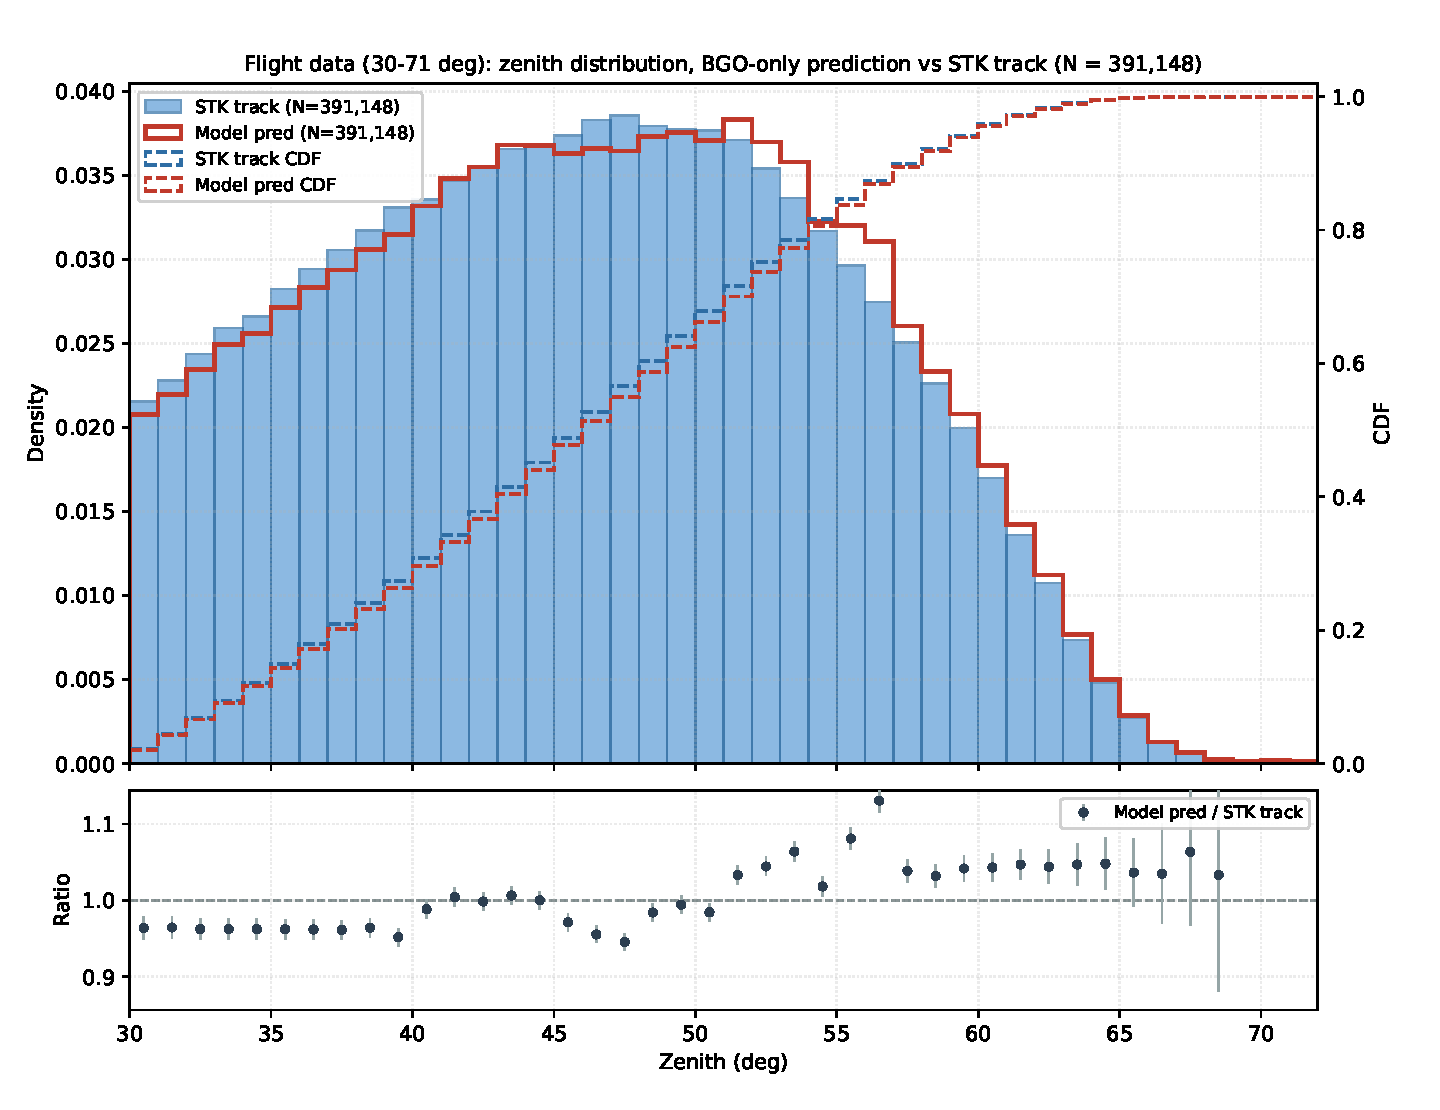
\includegraphics[width=0.85\textwidth]{graph_update/flight_zenith.pdf}
  \caption{Comparison of the zenith-angle distributions reconstructed by the
  BGO-only model and by the STK for flight electron candidates with both
  detectors traversed ($30^{\circ}\le\theta\le71^{\circ}$,
  $N=391{,}148$). \emph{Top}: filled blue histogram, STK track; red step
  line, model prediction (``Model pred'' in the legend), both normalized
  to unit area; the dashed blue and red curves are the corresponding
  cumulative distributions on the right-hand axis. \emph{Bottom}: ratio of
  the model prediction to the STK track in each $1^{\circ}$ zenith bin.
  The error bars give the statistical uncertainty
  $\sigma(R)/R=\sqrt{1/N_{\mathrm{pred}}+1/N_{\mathrm{STK}}}$; the dashed
  horizontal line marks unity. Only bins with at least 50 events in both
  samples are shown, and the two panels share the horizontal axis.}
  \label{fig:flight_zenith}
\end{figure}

\begin{figure}[htbp]
  \centering
  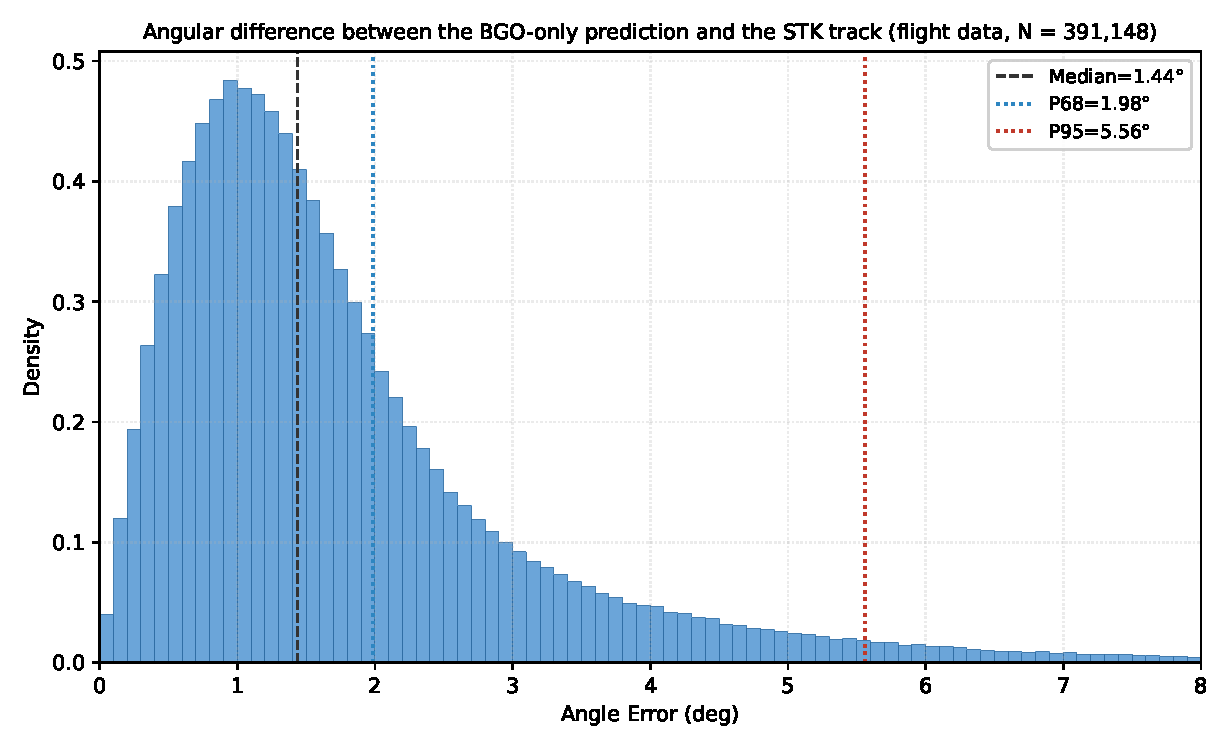
\includegraphics[width=0.85\textwidth]{graph_update/flight_angle_error_30_71.pdf}
  \caption{Distribution of the space-angle difference $\psi$ between the
  BGO-only model prediction and the STK track for the flight sample of
  Figure~\ref{fig:flight_zenith}. The dashed, dotted and dash-dotted vertical
  lines mark the median ($1.44^{\circ}$), the 68th percentile ($1.98^{\circ}$)
  and the 95th percentile ($5.56^{\circ}$), respectively. This quantity
  describes the agreement between two reconstructions. The STK track is
  not a truth direction, so $\psi$ is not an absolute angular resolution.}
  \label{fig:flight_angerr}
\end{figure}

Figure~\ref{fig:flight_energy} resolves the same quantity in
logarithmically equal-width bins of the BGO reconstructed energy between
$83.3$ and $941.2$~GeV. The median falls from $\sim 1.6^{\circ}$ in the
lowest bin to $\sim 1.2^{\circ}$ in the highest, and the 68th percentile
from $\sim 2.2^{\circ}$ to $\sim 1.6^{\circ}$. The 95th percentile declines
more gently, from $\sim 5.9^{\circ}$ to $\sim 5.1^{\circ}$, and shows
bin-to-bin scatter of up to $\sim 0.8^{\circ}$, while the number of entries
per bin drops from $\sim 1.2\times10^{5}$ to a few thousand. The median and
the 68th percentile describe the bulk of the events and change smoothly
with energy; the 95th percentile is set by a small subpopulation of poorly
reconstructed events (events misrouted near the $60^{\circ}$ boundary,
events with degraded STK track quality at large zenith angles, and residual
contamination), whose fraction can differ from bin to bin. Fewer events
widen the statistical uncertainty of this tail quantile in the highest
bins, but the largest excursions appear in bins with ample statistics, so
the finite bin population does not by itself explain the scatter. We do
not assign a single cause to it in the present analysis.

\begin{figure}[htbp]
  \centering
  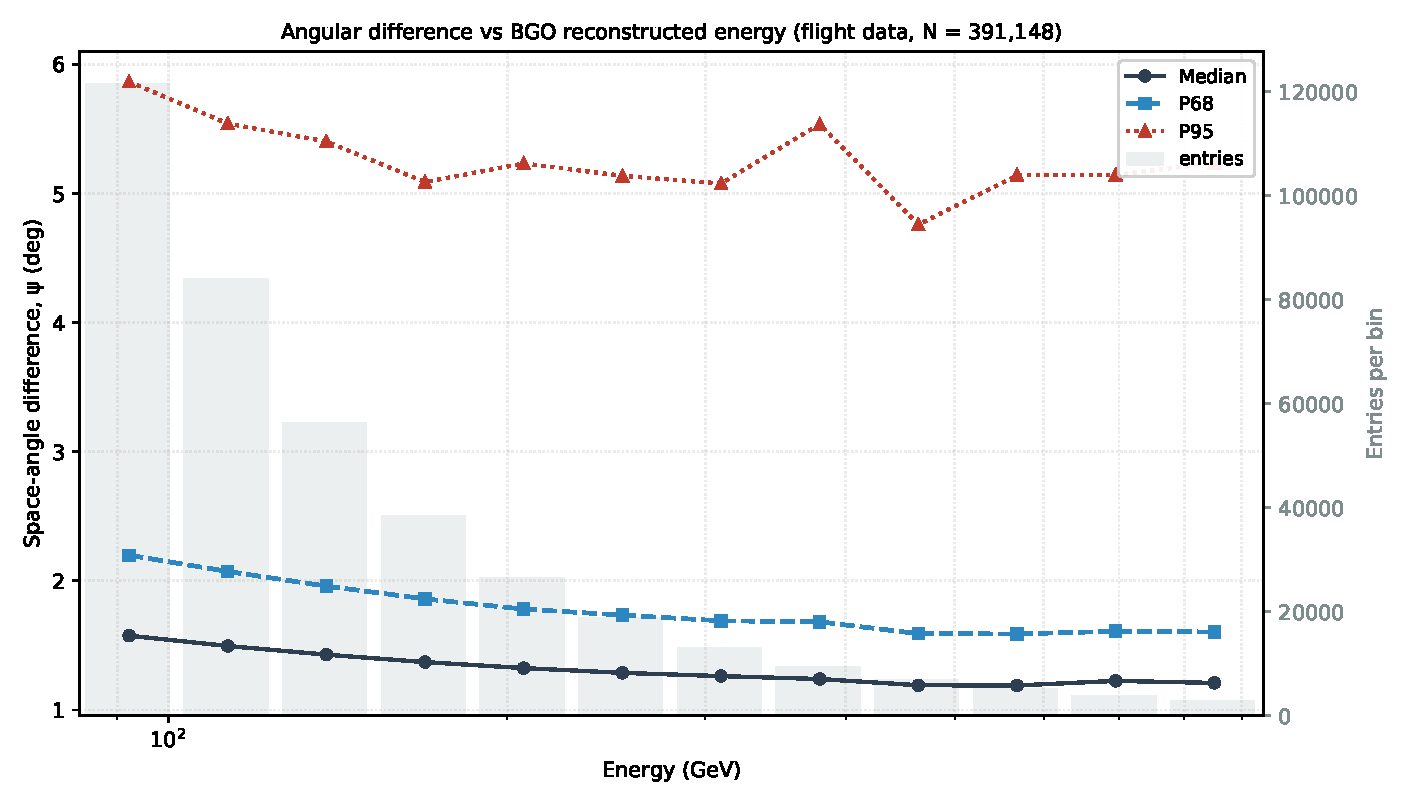
\includegraphics[width=0.85\textwidth]{graph_update/flight_error_vs_energy.pdf}
  \caption{Energy dependence of the space-angle difference between the
  BGO-only prediction and the STK track ($N=391{,}148$), binned in
  logarithmically equal-width intervals of the BGO reconstructed energy
  between 83.3 and 941.2~GeV. Black circles: median; blue squares: 68th
  percentile; red triangles: 95th percentile (left axis). Grey bars show
  the number of events per energy bin (right axis). The 95th percentile
  declines mildly with energy and shows bin-to-bin scatter on top of that
  trend. As a tail statistic, it responds more strongly than the median or
  the 68th percentile to the small subpopulation of poorly reconstructed
  events.}
  \label{fig:flight_energy}
\end{figure}

The STK track has a finite angular resolution of its own and is not a truth
label. We use $\psi$ to compare the BGO-only prediction with that track, so
the values reported above describe how well two reconstructions agree; the
absolute angular resolution of the BGO-only model cannot be determined
from this sample. The flight sample contains only events with an STK track,
and its energy spectrum and zenith distribution differ from the isotropic,
power-law Monte Carlo sample of Section~\ref{sec:data}. The 68th percentile
of $1.98^{\circ}$ is measured on this sample against the STK track and is
not directly comparable to the Monte Carlo $\Psi_{68}$ of $1.40^{\circ}$
and $1.31^{\circ}$. A difference between the flight and Monte Carlo values
would not, on its own, indicate a degradation or confirm the simulation.
The comparison shows degree-level agreement between the BGO-only predictions
and an independent tracker-based direction, and Figure~\ref{fig:flight_zenith}
shows no gross distortion of the zenith distribution. The energy trend in
Figure~\ref{fig:flight_energy} resembles that of
Figure~\ref{fig:resolution_energy}. The sample does not extend into the
$71^{\circ}$--$90^{\circ}$ region where the STK is blind and which motivates
the large-angle branch. The $60^{\circ}$--$71^{\circ}$ events that retain an
STK track form a biased subset of the large-angle population. The dedicated
study of detector effects (dead channels, pedestal and electronic noise,
gain drift and pile-up) and the full data/MC closure test on an unbiased
control sample remain ongoing. We expect the hemisphere assumption of
Section~\ref{ssec:large} to hold over the validated $0^{\circ}$--$90^{\circ}$
range, and we will revisit it when extending the reconstruction to
upward-going events.

\subsection{Physics Impact}

The primary scientific motivation for developing this full-angle reconstruction framework is to maximize the scientific yield of the DAMPE mission by expanding its effective observation window.

\textbf{Acceptance Enhancement:} The standard reconstruction pipeline, constrained by the geometric requirements of the STK and PSD, effectively utilizes only a limited fraction of the potential field of view of the BGO calorimeter. To quantify the gain from extending reliable BGO-only reconstruction from the conventional $60^{\circ}$ operating range to the full $90^{\circ}$ hemisphere, we compute the \emph{geometric acceptance} of the DAMPE BGO calorimeter for an isotropic cosmic-ray flux. Unlike a ground-based experiment, in which a flat detector module views the sky through a $\cos\theta$ projected-area weighting, DAMPE is a free-flying, six-faced box: a particle can enter through the top face \emph{or} any of the four side faces, so the acceptance must be evaluated from the full projected area of the box rather than from a single top-face projection. For a rectangular box of dimensions $L_x\times L_y\times L_z$, the Cauchy projection formula gives the projected area along a direction $(\theta,\phi)$ as
\begin{equation}
A_{\rm proj}(\theta,\phi)=L_xL_y\cos\theta+L_xL_z|\sin\theta\sin\phi|+L_yL_z|\sin\theta\cos\phi|,
\label{eq:proj}
\end{equation}
where the first term is the (top) face, visible for $\theta<90^{\circ}$, and the remaining two terms are the four side faces. The geometric acceptance within zenith angle $\theta_{\max}$ is the integral of this projected area over the solid angle,
\begin{multline}
G(\theta_{\max})=\int_{0}^{2\pi}\!\!\int_{0}^{\theta_{\max}}A_{\rm proj}(\theta,\phi)\,\sin\theta\,d\theta\,d\phi \\
=\pi L_xL_y\sin^{2}\theta_{\max}+2L_z(L_x+L_y)\bigl(\theta_{\max}-\sin\theta_{\max}\cos\theta_{\max}\bigr).
\label{eq:gf}
\end{multline}
The DAMPE BGO calorimeter comprises 308 BGO bars arranged in 14 layers of 22 bars in orthogonally alternating orientation, each bar measuring $2.5\times2.5\times60\ {\rm cm}^{3}$. Its active bounding box therefore has transverse dimensions $L_x=60\ {\rm cm}$ (bar length) and $L_y=22\times2.5=55\ {\rm cm}$ (packed width of one layer), and depth $L_z=14\times2.5=35\ {\rm cm}$ (corresponding to $\sim31$ radiation lengths). Adopting the conventional reliable limit $\theta_{c}\approx60^{\circ}$, beyond which the STK fiducial volume is progressively bypassed (consistent with the in-flight performance of the DAMPE silicon tracker~\cite{dampe_stk_perf}), the acceptance ratio to the full $90^{\circ}$ hemisphere is
\begin{equation}
\frac{G(90^{\circ})}{G(60^{\circ})}
=\frac{\pi L_xL_y+2L_z(L_x+L_y)\,\pi/2}
{\pi L_xL_y\sin^{2}60^{\circ}+2L_z(L_x+L_y)\bigl(\pi/3-\sin60^{\circ}\cos60^{\circ}\bigr)}
\approx 1.81.
\label{eq:gf_stk}
\end{equation}
The quantity that a physics analysis actually gains is the \emph{effective} acceptance, i.e.\ the geometric acceptance weighted by the probability that an event is reconstructed with a usable direction. Equation~(\ref{eq:gf_stk}) is the ratio of effective acceptances under the assumption that the conventional BGO+STK chain is fully efficient below $\theta_{c}$ and contributes nothing above it, while the new chain is fully efficient everywhere. The second assumption is borne out by the measured efficiencies of $99.47\%$ in $30^{\circ}$--$60^{\circ}$ and $99.50\%$ in $60^{\circ}$--$90^{\circ}$ (Table~\ref{tab:efficiency}). We therefore quote $\approx 1.8$ as the headline acceptance gain, understood as an effective-acceptance ratio rather than a purely geometric one. Equivalently, the newly accessible $60^{\circ}$--$90^{\circ}$ annulus alone contributes a geometric acceptance equal to $\sim 80\%$ of the previously covered $0^{\circ}$--$60^{\circ}$ range. This $\sim 1.8\times$ increase in statistics is valuable for studies of rare events, such as the search for monochromatic gamma-ray lines or the precise measurement of the cosmic ray electron spectrum at TeV energies, where the flux is extremely low and statistical uncertainty is the dominant error source.

\textbf{Background Rejection:} The improved trajectory reconstruction also has implications for particle identification, specifically electron--proton discrimination, which relies heavily on analyzing the three-dimensional shower morphology relative to the shower axis. A precise axis reconstruction allows for a more accurate definition of the ``shower core'' and ``isolation cone,'' which are central to the calculation of rejection variables. By providing a reliable track even for large-angle events, the method extends the domain over which electron--proton separation algorithms can operate, opening the high-inclination regime to the same discrimination tools already used near normal incidence. We note that this is a forward-looking capability: a dedicated quantitative rejection study on a mixed proton--electron Monte Carlo sample, including the definition of appropriate shower-core and isolation-cone variables in the large-angle regime, has not yet been performed and is deferred to future work.

\subsection{Systematic Uncertainties and Monte Carlo Limitations}
\label{ssec:systematics}

The resolution and efficiency values reported above come from GEANT4
simulation. The flight-data comparison of Section~\ref{ssec:flight} checks
the reconstructed directions against STK tracks, which are not truth labels,
so it does not replace a data/MC closure test. Real detector conditions add
effects that the nominal simulation omits: dead or noisy channels, pedestal
and electronic noise, gain drift over the mission lifetime, and pile-up at
high rates. We inject representative detector effects into the simulation
and re-evaluate the angular resolution and efficiency. Under the injected
perturbations the standard-angle resolution degrades from $1.40^{\circ}$ to
$1.52^{\circ}$, and the large-angle resolution from $1.31^{\circ}$ to
$1.66^{\circ}$; the efficiency stays above $98.0\%$ in both regimes. These
preliminary numbers suggest that the reconstruction tolerates realistic
detector perturbations. A full data/MC closure test on an unbiased
flight-data control sample remains the definitive validation and is ongoing.
Until that comparison is available, the absolute resolution figures should
be read as Monte Carlo projections. The dependence of the shower model on
the Geant4 physics list has not been explored systematically.

\subsection{Limitations and Uncertainty Quantification}
\label{ssec:limitations}

\textbf{Scope limitations.} The present validation is restricted to electron primaries in the 100 GeV--1 TeV energy range and the $0^{\circ}$--$90^{\circ}$ zenith band. The flight-data cross-check covers only events with an STK track in the $30^{\circ}$--$71^{\circ}$ range, and it leaves the STK-blind region above $71^{\circ}$ untested. The scientific motivation (TeV electron spectra, gamma-ray lines) extends to higher energies, and the complementary proton, helium, and heavier-nuclei channels, as well as the upward-going $90^{\circ}$--$130^{\circ}$ regime, are explicitly deferred to future work. Consequently, the acceptance gain and resolution figures should not be extrapolated beyond the validated electron / 100 GeV--1 TeV / $0^{\circ}$--$90^{\circ}$ domain without further study.

\textbf{Input-engineering choices.} The thresholds used in the large-angle five-channel input (100\,GeV saturation flag and 500\,MeV low-energy clip) are empirical engineering choices that were found to improve reconstruction quality on the 100\,GeV--1\,TeV electron sample. They are not derived from first-principles detector calibration, and their optimal values may differ for other primary species or energy regimes. A systematic threshold scan is outside the scope of the present work and remains useful future work.

\textbf{Direction uncertainty quantification.} The reported $\Psi_{68}$ is an empirical 68\% containment radius of the space-angle error distribution; across the energy bins of Figure~\ref{fig:resolution_energy} it is well calibrated and shows no strong energy trend (particularly for the standard-angle branch, where it is essentially flat), so the per-energy $\Psi_{68}$ values are already approximate confidence intervals. We have not yet implemented per-event predictive uncertainty (e.g., the Bayesian uncertainty decomposition of Kendall and Gal~\cite{kendall_2017}); such an extension would provide event-level error bars useful for source-morphology and line-search analyses and is a natural next step.

\section{Conclusion}
\label{sec:conclusion}

In this work, we have proposed and validated a hierarchical framework for particle trajectory reconstruction up to $90^{\circ}$ in the BGO calorimeter with DAMPE experiment. Addressing the principal limitation of conventional methods, which fail for large-angle events due to geometric constraints, the hierarchical deep learning strategy effectively decouples the reconstruction from the auxiliary detectors (STK).

Our approach uses a ``divide-and-conquer'' strategy, with a high-precision SVM classifier that routes events to specialized reconstruction branches. For standard incidence angles ($0^{\circ}$--$60^{\circ}$), the PGHNN synergizes analytical physical priors with data-driven features, achieving an angular resolution of $1.40^{\circ}$ with BGO data alone and superior stability against energy fluctuations compared to standard algorithms. For large incidence angles ($60^{\circ}$--$90^{\circ}$), where analytical methods collapse, the DLD model successfully recovers the trajectory information from truncated shower topologies, maintaining a resolution of $1.31^{\circ}$. Collectively, this framework achieves nearly 100\% reconstruction efficiency across the entire angular domain for electrons in the 100~GeV to 1~TeV range, raising the effective acceptance of the detector by a factor of $\approx 1.8$. Applied to flight electron candidates with STK tracks ($30^{\circ}$--$71^{\circ}$), the predicted directions agree with the STK tracks at the degree level (median $1.44^{\circ}$, 68th percentile $1.98^{\circ}$). This is a consistency check between two reconstructions: the STK track has its own finite resolution and is not a truth direction, so the comparison does not yield an absolute angular resolution of the BGO-only model.

Looking forward, this work points to several concrete research directions. First, we aim to extend the angular coverage of the reconstruction framework beyond the current $0^{\circ}$--$90^{\circ}$ range to include grazing and upward-going events in the $90^{\circ}$--$130^{\circ}$ regime. In this range, particles enter the detector from below the horizon, traversing the BGO calorimeter in the reverse direction and producing fundamentally different shower topologies characterized by asymmetric energy deposition. Extending the DLD architecture to handle these inverted geometries will further expand the effective field of view of the detector and improve the sensitivity to upward-going cosmic-ray and Earth-albedo events. Second, we aim to extend this methodology beyond the electron to include nucleon cosmic rays, such as protons, helium, and heavier nuclei (C, Mg, Fe). Reconstructing these species solely with the calorimeter is challenging due to the complexity of hadronic showers, but it is essential for extending the spectral measurements to the PeV range where statistics are scarce. Third, we plan to explore a unified, multi-task learning architecture capable of simultaneous trajectory reconstruction and energy estimation. By sharing feature extraction backbones, such a model could not only improve computational efficiency for on-board processing but also use the mutual correlations between spatial and calorimetric features to further improve overall precision.


\section*{Data and Code availability}
The authors do not have permission to share data. But the code to train and evaluate models is available at \url{https://github.com/kelly-struck/Electron-Trajectory-Reconstruction.git}. 

\section*{Acknowledgments}
The DAMPE mission was funded by the strategic priority science and technology projects in space science of Chinese Academy of Sciences (CAS). In China, the data analysis was supported by the National Key Research and Development Program of China (No. 2022YFF0503302), we acknowledge the support from the National Natural Science Foundation of China (No. 12227805). We also thank W. H. Li for simulation data selection and helpful discussion with S. J. Lei.

% %% Use a table environment to create tables.
% %% Refer following link for more details.
% %% https://en.wikibooks.org/wiki/LaTeX/Tables
% \begin{table}[t]%% placement specifier
% %% Use tabular environment to tag the tabular data.
% %% https://en.wikibooks.org/wiki/LaTeX/Tables#The_tabular_environment
% \centering%% For centre alignment of tabular.
% \begin{tabular}{l c r}%% Table column specifiers
% %% Tabular cells are separated by &
%   1 & 2 & 3 \\ %% A tabular row ends with \\
%   4 & 5 & 6 \\
%   7 & 8 & 9 \\
% \end{tabular}
% %% Use \caption command for table caption and label.
% \caption{Table Caption}\label{fig1}
% \end{table}


% %% Use figure environment to create figures
% %% Refer following link for more details.
% %% https://en.wikibooks.org/wiki/LaTeX/Floats,_Figures_and_Captions
% \begin{figure}[t]%% placement specifier
% %% Use \includegraphics command to insert graphic files. Place graphics files in 
% %% working directory.
% \centering%% For centre alignment of image.
% \includegraphics{example-image-a}
% %% Use \caption command for figure caption and label.
% \caption{Figure Caption}\label{fig1}
% %% https://en.wikibooks.org/wiki/LaTeX/Importing_Graphics#Importing_external_graphics
% \end{figure}


% %% The Appendices part is started with the command \appendix;
% %% appendix sections are then done as normal sections
% \appendix
% \section{Example Appendix Section}
% \label{app1}

% Appendix text.

% %% For citations use: 
% %%       \cite{<label>} ==> [1]

% %%
% Example citation, See \cite{lamport94}.

% %% If you have bib database file and want bibtex to generate the
% %% bibitems, please use
% %%
% %%  \bibliographystyle{elsarticle-num} 
% %%  \bibliography{<your bibdatabase>}

% %% else use the following coding to input the bibitems directly in the
% %% TeX file.

% %% Refer following link for more details about bibliography and citations.
% %% https://en.wikibooks.org/wiki/LaTeX/Bibliography_Management

\begin{thebibliography}{00}
\bibitem{dampe_mission}
  J. Chang et al.,
  \textit{The dark matter particle explorer mission},
  Astropart. Phys., vol.~95, pp.~6--24, 2017.
  \doi{10.1016/j.astropartphys.2017.08.005}

\bibitem{ambrosi_2017}
  G. Ambrosi et al.,
  \textit{Direct detection of a break in the teraelectronvolt cosmic-ray spectrum of electrons and positrons},
  Nature, vol.~552, pp.~63--66, 2017.
  \doi{10.1038/nature24475}

\bibitem{an_2019}
  Q. An et al.,
  \textit{Measurement of the cosmic-ray proton spectrum from 40 GeV to 100 TeV with the DAMPE satellite},
  Sci. Adv., vol.~5, no.~9, p.~eaax3793, 2019.
  \doi{10.1126/sciadv.aax3793}

\bibitem{alemanno_helium_2021}
  F. Alemanno et al.,
  \textit{Measurement of the cosmic ray helium energy spectrum from 70 GeV to 80 TeV with the DAMPE space mission},
  Phys. Rev. Lett., vol.~126, no.~20, p.~201102, 2021.
  \doi{10.1103/PhysRevLett.126.201102}

\bibitem{alemanno_p_he_2024}
  F. Alemanno et al. (DAMPE Collaboration),
  \textit{Measurement of the cosmic $p+\mathrm{He}$ energy spectrum from 50 GeV to 0.5 PeV with the DAMPE space mission},
  Phys. Rev. D, vol.~109, no.~12, p.~L121101, 2024.
  \doi{10.1103/PhysRevD.109.L121101}

\bibitem{alemanno_proton_iron_2025}
  F. Alemanno et al.,
  \textit{Charge-dependent spectral softenings of primary cosmic-rays from proton to iron below the knee},
  arXiv preprint arXiv:2511.05409, 2025.

\bibitem{li_2019}
  X. Li et al.,
  \textit{Recent gamma-ray results from DAMPE},
  in 36th International Cosmic Ray Conference (ICRC2019), vol.~36, p.~576, 2019.


  \doi{10.22323/1.358.0576}

\bibitem{dampe_psd_calib}
  M. Ding et al.,
  \textit{Calibration of the DAMPE plastic scintillator detector and its on-orbit performance},
  Res. Astron. Astrophys., vol.~19, no.~3, p.~047, 2019.
  \doi{10.1088/1674-4527/19/3/47}

\bibitem{dampe_psd_design}
  Y. Yu et al.,
  \textit{The plastic scintillator detector for DAMPE},
  Astropart. Phys., vol.~94, pp.~1--10, 2017.
  \doi{10.1016/j.astropartphys.2017.06.004}

\bibitem{dong_2019}
  T. Dong et al.,
  \textit{Charge measurement of cosmic ray nuclei with the plastic scintillator detector of DAMPE},
  Astropart. Phys., vol.~105, pp.~31--36, 2019.
  \doi{10.1016/j.astropartphys.2018.10.001}

\bibitem{ma_2019}
  P. Ma et al.,
  \textit{A method for aligning the plastic scintillator detector on DAMPE},
  Res. Astron. Astrophys., vol.~19, no.~6, p.~082, 2019.

  \doi{10.1088/1674-4527/19/6/82}

\bibitem{dampe_stk_perf}
  A. Tykhonov et al.,
  \textit{In-flight performance of the DAMPE silicon tracker},
  Nucl. Instrum. Methods A, vol.~924, pp.~309--315, 2019.
  \doi{10.1016/j.nima.2018.06.036}

\bibitem{dampe_stk_align}
  A. Tykhonov et al.,
  \textit{Internal alignment and position resolution of the silicon tracker of DAMPE determined with orbit data},
  Nucl. Instrum. Meth. A, vol.~893, pp.~43--56, 2018.
  \doi{10.1016/j.nima.2018.02.105}

\bibitem{dampe_stk_design}
  P. Azzarello et al.,
  \textit{The DAMPE Silicon--Tungsten tracker},
  Nucl. Instrum. Meth. A, vol.~831, pp.~378--384, 2016.
  \doi{10.1016/j.nima.2016.02.077}

\bibitem{dampe_bgo_beam}
  Y. Wei et al.,
  \textit{Performance of the DAMPE BGO calorimeter on the ion beam test},
  Nucl. Instrum. Methods A, vol.~922, pp.~177--184, 2019.
  \doi{10.1016/j.nima.2018.12.036}

\bibitem{dampe_bgo_calib}
  Z. Zhang et al.,
  \textit{The calibration and electron energy reconstruction of the BGO ECAL of the DAMPE detector},
  Nucl. Instrum. Methods A, vol.~836, pp.~98--104, 2016.
  \doi{10.1016/j.nima.2016.08.015}

\bibitem{dampe_bgo_readout}
  Y.-L. Zhang et al.,
  \textit{A high dynamic range readout unit for a calorimeter},
  Chin. Phys. C, vol.~36, no.~1, pp.~71--73, 2012.
  \doi{10.1088/1674-1137/36/1/012}

\bibitem{dampe_nud}
  Y.-Y. Huang et al.,
  \textit{Calibration and performance of the neutron detector onboard of the DAMPE mission},
  Res. Astron. Astrophys., vol.~20, p.~153, 2020.
  \doi{10.1088/1674-4527/20/9/153}

\bibitem{dampe_stk_soft}
  A. Tykhonov, V. Gallo, X. Wu, S. Zimmer,
  \textit{Reconstruction software of the silicon tracker of DAMPE mission},
  J. Phys. Conf. Ser., vol.~898, no.~4, p.~042031, 2017.
  \doi{10.1088/1742-6596/898/4/042031}

\bibitem{atwood_2009}
  W. B. Atwood et al.,
  \textit{The Large Area Telescope on the Fermi Gamma-ray Space Telescope Mission},
  Astrophys. J., vol.~697, no.~2, pp.~1071--1102, 2009.

  \doi{10.1088/0004-637X/697/2/1071}

\bibitem{asaoka_2019}
  Y. Asaoka et al.,
  \textit{The CALorimetric electron telescope (CALET) on the international space station: Results from the first two years on orbit},
  J. Phys. Conf. Ser., vol.~1181, no.~1, p.~012003, 2019.


  \doi{10.1088/1742-6596/1181/1/012003}

\bibitem{asaoka_cal_2017}
  Y. Asaoka et al.,
  \textit{Energy calibration of CALET onboard the International Space Station},
  Astroparticle Physics, vol.~91, pp.~1--10, 2017.
  \doi{10.1016/j.astropartphys.2017.03.002}

\bibitem{dampe_trigger_2019}
  Y.-Q. Zhang et al.,
  \textit{Design and on-orbit status of the trigger system for the DAMPE mission},
  Research in Astronomy and Astrophysics, vol.~19, no.~9, p.~123, 2019.
  \doi{10.1088/1674-4527/19/9/123}

\bibitem{liang_2022}
  Y.-F. Liang et al. (DAMPE Collaboration),
  \textit{Search for gamma-ray spectral lines with the DArk Matter Particle Explorer},
  Science Bulletin, vol.~67, no.~7, pp.~679--684, 2022.
  \doi{10.1016/j.scib.2021.12.015}

\bibitem{dampe_bgo_reco_status}
  L. Wu et al.,
  \textit{Calibration and status of the 3-D imaging calorimeter of DAMPE for cosmic ray physics on orbit},
  IEEE Trans. Nucl. Sci., vol.~65, no.~8, pp.~2007--2012, 2018.
  \doi{10.1109/TNS.2018.2814619}

\bibitem{lei_2019}
  S. J. Lei and W. Jiang,
  \textit{BGO Track Reconstruction with DAMPE},
  in 36th International Cosmic Ray Conference (ICRC2019), vol.~36, p.~329, 2019.
  \doi{10.22323/1.358.0329}


  \doi{10.1088/1748-0221/11/09/P09001}

\bibitem{paganini_2018}
  M. Paganini, L. de Oliveira, and B. Nachman,
  \textit{CaloGAN: Simulating 3D high energy particle showers in multilayer electromagnetic calorimeters with generative adversarial networks},
  Phys. Rev. D, vol.~97, no.~1, p.~014021, 2018.

  \doi{10.1103/PhysRevD.97.014021}

\bibitem{erdmann_2018}
  M. Erdmann, J. Glombitza, and D. Walz,
  \textit{A deep learning-based reconstruction of cosmic ray-induced air showers},
  Astroparticle Physics, vol.~97, pp.~46--53, 2018.
  \doi{10.1016/j.astropartphys.2017.10.006}

\bibitem{guillen_2019}
  A. Guill\'en et al.,
  \textit{Deep learning techniques applied to the physics of extensive air showers},
  Astroparticle Physics, vol.~111, pp.~12--22, 2019.
  \doi{10.1016/j.astropartphys.2019.03.001}

\bibitem{yang_2024}
  X.~G. Yang, Z. Quan, Y.~W. Dong, M. Xu, C. Zhang, J.~J. Wang, C.~L. Liao, Q. Wu, J.~Y. Sun, X. Liu, R.~J. Wang, Z.~G. Wang, and B.~B. Wu,
  \textit{Application of a deep learning method for shower axis reconstruction in a 3D imaging calorimeter},
  Nucl. Instrum. Methods A, vol.~1066, p.~169571, 2024.
  \doi{10.1016/j.nima.2024.169571}

\bibitem{carleo_2019}
  G. Carleo et al.,
  \textit{Machine learning and the physical sciences},
  Rev. Modern Phys., vol.~91, p.~045002, 2019.
  \doi{10.1103/RevModPhys.91.045002}

\bibitem{seyyedi_2023}
  A. Seyyedi, M. Bohlouli, and S. N. Oskoee,
  \textit{Machine learning and physics: A survey of integrated models},
  ACM Computing Surveys, vol.~56, no.~5, pp.~1--33, 2023.
  \doi{10.1145/3611383}

\bibitem{meng_2025}
  C. Meng, S. Griesemer, D. Cao, et al.,
  \textit{When physics meets machine learning: A survey of physics-informed machine learning},
  Machine Learning for Computational Science and Engineering, vol.~1, no.~1, p.~20, 2025.
  \doi{10.1007/s44379-025-00016-0}

\bibitem{lecun_2015}
  Y. LeCun, Y. Bengio, and G. Hinton,
  \textit{Deep learning},
  Nature, vol.~521, pp.~436--444, 2015.
  \doi{10.1038/nature14539}

\bibitem{tykhonov_2023}
  A. Tykhonov, A. Kotenko, P. Coppin, et al.,
  \textit{A deep learning method for the trajectory reconstruction of cosmic rays with the DAMPE mission},
  Astroparticle Physics, vol.~146, p.~102795, 2023.
  \doi{10.1016/j.astropartphys.2022.102795}

\bibitem{karpatne_2017}
  A. Karpatne, G. Atluri, J. H. Faghmous, et al.,
  \textit{Theory-guided data science: A new paradigm for scientific discovery from data},
  IEEE Transactions on Knowledge and Data Engineering, vol.~29, no.~10, pp.~2318--2331, 2017.
  \doi{10.1109/TKDE.2017.2720168}

\bibitem{kerrigan_2021}
  D. Kerrigan, J. Hullman, and E. Bertini,
  \textit{A survey of domain knowledge elicitation in applied machine learning},
  Multimodal Technol. Interact., vol.~5, no.~12, p.~73, 2021.

  \doi{10.3390/mti5120073}

\bibitem{karniadakis_2021}
  G. E. Karniadakis, I. G. Kevrekidis, L. Lu, et al.,
  \textit{Physics-informed machine learning},
  Nature Reviews Physics, vol.~3, no.~6, pp.~422--440, 2021.

  \doi{10.1038/s42254-021-00314-5}

\bibitem{willard_2022}
  J. Willard, X. Jia, S. Xu, M. Steinbach, and V. Kumar,
  \textit{Integrating scientific knowledge with machine learning for engineering and environmental systems},
  ACM Computing Surveys, vol.~55, no.~4, pp.~1--37, 2022.
  \doi{10.1145/3514228}

\bibitem{cortes_1995}
  C. Cortes and V. Vapnik,
  \textit{Support-vector networks},
  Machine learning, vol.~20, no.~3, pp.~273--297, 1995.
  \doi{10.1007/BF00994018}

\bibitem{geant4_2016}
  John Allison et al.,
  \textit{Recent developments in Geant4},
  Nuclear Instruments and Methods in Physics Research Section A,
  vol.~835, pp.~186--225,
  2016.

  \doi{10.1016/j.nima.2016.06.125}

\bibitem{ftfp_model1}
  Bo Andersson, G{\"o}sta Gustafson, and Bo Nilsson-Almqvist,
  \textit{A model for low-pt hadronic reactions with generalizations to hadron-nucleus and nucleus-nucleus collisions},
  Nuclear Physics B,
  vol.~281, no.~1--2, pp.~289--309,
  1987.
  \doi{10.1016/0550-3213(87)90257-4}

\bibitem{ftfp_model2}
  Bo Nilsson-Almqvist and E. Stenlund,
  \textit{Interactions between hadrons and nuclei: The lund Monte Carlo-FRITIOF version 1.6},
  Computer Physics Communications,
  vol.~43, no.~3, pp.~387--397,
  1987.
  \doi{10.1016/0010-4655(87)90056-7}

\bibitem{bertini_cascade}
  Dennis Wright and Michael Kelsey,
  \textit{The Geant4 bertini cascade},
  Nuclear Instruments and Methods in Physics Research Section A,
  vol.~804, pp.~175--188,
  2015.


  \doi{10.1016/j.nima.2015.09.058}

% \bibitem{jacobs_1991}
%   R. A. Jacobs, M. I. Jordan, S. J. Nowlan, and G. E. Hinton,
%   \textit{Adaptive mixtures of local experts},
%   Neural Computation, vol.~3, no.~1, pp.~79--87, 1991.
%   \doi{10.1162/neco.1991.3.1.79}

\bibitem{pedregosa_2011}
  F. Pedregosa et al.,
  \textit{Scikit-learn: Machine Learning in Python},
  Journal of Machine Learning Research, vol.~12, pp.~2825--2830, 2011.

\bibitem{he2016deep}
  K. He, X. Zhang, S. Ren, and J. Sun,
  \textit{Deep residual learning for image recognition},
  in \textit{Proceedings of the IEEE Conference on Computer Vision and Pattern Recognition (CVPR)},
  pp.~770--778,
  2016.
  \doi{10.1109/CVPR.2016.90}

\bibitem{woo2018cbam}
  S. Woo, J. Park, J.-Y. Lee, and I. S. Kweon,
  \textit{CBAM: Convolutional Block Attention Module},
  in \textit{Proceedings of the European Conference on Computer Vision (ECCV)}, pp.~3--19, 2018.

  \doi{10.1007/978-3-030-01234-2_1}

\bibitem{szegedy2016rethinking}
  C. Szegedy, V. Vanhoucke, S. Ioffe, J. Shlens, and Z. Wojna,
  \textit{Rethinking the inception architecture for computer vision},
  in \textit{Proceedings of the IEEE Conference on Computer Vision and Pattern Recognition (CVPR)},
  pp.~2818--2826,
  2016.
  \doi{10.1109/CVPR.2016.308}

\bibitem{wang2009mse}
  Z. Wang and A. C. Bovik,
  \textit{Mean squared error: Love it or leave it? A new look at signal fidelity measures},
  IEEE Signal Processing Magazine,
  vol.~26, no.~1, pp.~98--117,
  2009.
  \doi{10.1109/MSP.2008.930649}

\bibitem{bengio_2009}
  Y. Bengio, J. Louradour, R. Collobert, and J. Weston,
  \textit{Curriculum learning},
  in Proceedings of the 26th Annual International Conference on Machine Learning, pp.~41--48, 2009.
  \doi{10.1145/1553374.1553380}

\bibitem{kendall_2017}
  A. Kendall and Y. Gal,
  \textit{What uncertainties do we need in Bayesian deep learning for computer vision?},
  in Advances in Neural Information Processing Systems (NIPS), vol.~30, 2017.
\end{thebibliography}

\end{document}